\documentclass[conference]{IEEEtran}
\usepackage{amsmath}
\usepackage{graphicx}
\usepackage{booktabs}
\usepackage{cite}
\usepackage{url}
% Figures are produced by the Phase 2 pipeline in figures/phase2/ (../ locally, ./ on Overleaf).
\graphicspath{{../figures/phase2/}{figures/phase2/}}
% Every number quoted in the text is a macro generated from the results files:
%   python report/build_phase2_report_assets.py
% Generated by report/build_phase2_report_assets.py. Do not edit by hand.
\newcommand{\ValPoneRecipeOne}{0.9343}
\newcommand{\ValPoneRecipeOneStd}{0.0023}
\newcommand{\ValPoneRecipeOneGap}{2.74}
\newcommand{\ValPoneRecipeTwo}{0.9314}
\newcommand{\ValPoneRecipeTwoStd}{0.0011}
\newcommand{\ValPoneRecipeTwoGap}{0.29}
\newcommand{\ValPlain}{0.9510}
\newcommand{\ValPlainStd}{0.0024}
\newcommand{\ValPlainGap}{1.74}
\newcommand{\ValBase}{0.9523}
\newcommand{\ValBaseStd}{0.0007}
\newcommand{\ValBaseGap}{1.49}
\newcommand{\ValDeeper}{0.9557}
\newcommand{\ValDeeperStd}{0.0010}
\newcommand{\ValDeeperGap}{2.53}
\newcommand{\ValNoAugGap}{5.35}
\newcommand{\ValNoAugTrainAcc}{0.9990}
\newcommand{\ValPoneRecipeTwoTrainAcc}{0.9347}
\newcommand{\RecipeOnPoneDelta}{-0.28}
\newcommand{\RecipeOnPoneAllNegative}{all three}
\newcommand{\ArchGainSameRecipe}{+1.96}
\newcommand{\BaseVsPoneGain}{+1.80}
\newcommand{\DeltaDeeper}{+0.34}
\newcommand{\DeltaNarrow}{-1.10}
\newcommand{\DeltaNoBN}{-0.70}
\newcommand{\DeltaPlain}{-0.13}
\newcommand{\DeltaNoErase}{-0.16}
\newcommand{\DeltaNoFlip}{+0.00}
\newcommand{\DeltaNoAug}{-0.72}
\newcommand{\DeltaConstLR}{-0.68}
\newcommand{\DeltaSGD}{-0.09}
\newcommand{\DeltaDropHalf}{-0.18}
\newcommand{\DeltaDropZero}{+0.02}
\newcommand{\DeltaNoLS}{-0.29}
\newcommand{\DeltaNoWD}{-0.10}
\newcommand{\NoBNStd}{0.50}
\newcommand{\BaseStdPP}{0.07}
\newcommand{\ShortcutGain}{+0.13}
\newcommand{\GainLS}{0.29}
\newcommand{\NRuns}{48}
\newcommand{\NConfigs}{16}
\newcommand{\TrainMinutesTotal}{105}
\newcommand{\TrainSecondsDeeper}{225}
\newcommand{\TrainSecondsPone}{49}
\newcommand{\ParamsPone}{241,546}
\newcommand{\ParamsBase}{308,074}
\newcommand{\ParamsDeeper}{696,042}
\newcommand{\ParamsNarrow}{77,754}
\newcommand{\DenseSharePone}{61.6}
\newcommand{\RFPone}{22}
\newcommand{\RFBase}{34}
\newcommand{\RFDeeper}{62}
\newcommand{\FinalName}{arch\_deeper}
\newcommand{\TestPone}{0.9252}
\newcommand{\TestPoneStd}{0.0034}
\newcommand{\TestPoneF}{0.9250}
\newcommand{\TestPoneShirt}{0.757}
\newcommand{\TestPoneInGroup}{12.2}
\newcommand{\TestFinal}{0.9488}
\newcommand{\TestFinalStd}{0.0015}
\newcommand{\TestFinalF}{0.9487}
\newcommand{\TestFinalShirt}{0.834}
\newcommand{\TestFinalInGroup}{8.5}
\newcommand{\TestHone}{0.9495}
\newcommand{\TestHoneStd}{0.0009}
\newcommand{\TestHoneF}{0.9494}
\newcommand{\TestHoneShirt}{0.833}
\newcommand{\TestHoneInGroup}{8.4}
\newcommand{\TestHtwo}{0.9502}
\newcommand{\TestHtwoStd}{0.0020}
\newcommand{\TestHtwoF}{0.9501}
\newcommand{\TestHtwoShirt}{0.839}
\newcommand{\TestHtwoInGroup}{8.3}
\newcommand{\TestHthree}{0.9502}
\newcommand{\TestHthreeStd}{0.0021}
\newcommand{\TestHthreeF}{0.9501}
\newcommand{\TestHthreeShirt}{0.839}
\newcommand{\TestHthreeInGroup}{8.3}
\newcommand{\TestHzero}{0.9048}
\newcommand{\TestHzeroStd}{0.0000}
\newcommand{\TestHzeroF}{0.9047}
\newcommand{\TestHzeroShirt}{0.708}
\newcommand{\TestHzeroInGroup}{15.3}
\newcommand{\TestFinalCILow}{0.9445}
\newcommand{\TestFinalCIHigh}{0.9532}
\newcommand{\TestGainFinalVsPone}{+2.36}
\newcommand{\ErrorsPoneMean}{748}
\newcommand{\ErrorsFinalMean}{512}
\newcommand{\ErrorReduction}{32}
\newcommand{\HtwoGain}{+0.15}
\newcommand{\HtwoGainMin}{+0.11}
\newcommand{\HtwoGainMax}{+0.22}
\newcommand{\HoneGain}{+0.08}
\newcommand{\HtwoGainVal}{+0.21}
\newcommand{\HzeroVal}{0.9162}
\newcommand{\PHtwoVsFinal}{0.20}
\newcommand{\PHoneVsFinal}{0.23}
\newcommand{\PHtwoVsHone}{0.90}
\newcommand{\McFinalOnly}{367}
\newcommand{\McPoneOnly}{158}
\newcommand{\McHtwoOnly}{36}
\newcommand{\McFinalOnlyVsHtwo}{25}
\newcommand{\NComparisons}{7}
\newcommand{\CompHogFixes}{181}
\newcommand{\CompCnnErrors}{510}
\newcommand{\CompHogFixShare}{35.5}
\newcommand{\CompOracle}{0.9671}
\newcommand{\RoutedTest}{5.7}
\newcommand{\RoutedVal}{5.4}
\newcommand{\Tau}{0.7}
\newcommand{\HtwoAlpha}{2}
\newcommand{\HtwoDim}{128}
\newcommand{\HtwoC}{1}
\newcommand{\PcaVar}{48.3}
\newcommand{\NGateModels}{16}
\newcommand{\FreezeSha}{a6eb05ea62db}
\newcommand{\PhaseOneCnnAcc}{0.9274}
\newcommand{\PhaseOneHogSvmAcc}{0.8817}
\newcommand{\PhaseOneSvmAcc}{0.8953}
\newcommand{\PhaseOneShirt}{0.747}
\newcommand{\EceFinalTest}{0.067}
\newcommand{\EcePoneTest}{0.013}
\newcommand{\ConfFinalTest}{0.886}
\newcommand{\EceBaseVal}{0.083}
\newcommand{\EceNoLSVal}{0.010}
\newcommand{\RobNoiseP}{0.546}
\newcommand{\RobNoiseF}{0.167}
\newcommand{\RobNoiseH}{0.172}
\newcommand{\RobNoiseZ}{0.329}
\newcommand{\RobBrightP}{0.459}
\newcommand{\RobBrightF}{0.553}
\newcommand{\RobBrightH}{0.601}
\newcommand{\RobBrightZ}{0.890}
\newcommand{\RobContrastP}{0.793}
\newcommand{\RobContrastF}{0.868}
\newcommand{\RobContrastH}{0.869}
\newcommand{\RobContrastZ}{0.899}
\newcommand{\RobShiftP}{0.664}
\newcommand{\RobShiftF}{0.942}
\newcommand{\RobShiftH}{0.940}
\newcommand{\RobShiftZ}{0.416}
\newcommand{\RobOcclP}{0.836}
\newcommand{\RobOcclF}{0.916}
\newcommand{\RobOcclH}{0.914}
\newcommand{\RobOcclZ}{0.794}
\newcommand{\RobNoiseMidF}{0.381}
\newcommand{\RobNoiseMidP}{0.855}
\newcommand{\GpuMsPone}{0.011}
\newcommand{\GpuMsFinal}{0.077}
\newcommand{\CpuMsPone}{0.50}
\newcommand{\CpuMsFinal}{2.49}
\newcommand{\MsHtwo}{5.56}
\newcommand{\GpuSlowdown}{7.1}


\begin{document}

\title{Inventory Image Tagging via Handcrafted Features and a Small CNN\\
\large Phase 2: Deep Architecture, Ablation Studies and a Handcrafted--Learned Hybrid}

\author{\IEEEauthorblockN{Manas Selukar (2401010259), Anant Singh (2401010067), Akhil Sharma (2401020084),\\
Tanish Rao (2401010474), Rohan Kumar (2401020103), Puneet Takhar (2401010358)}
\IEEEauthorblockA{CSAI student project, Project 11: Automatic Clothing Category Recognition}}

\maketitle

\begin{abstract}
Phase 1 of this project compared eight classical models with a three-layer convolutional network (CNN) on
Fashion-MNIST; the CNN reached \PhaseOneCnnAcc{} test accuracy from a single training run and confused the
upper-body classes. Phase 2 studies the deep model itself. We design a residual network family with batch
normalisation and global average pooling, train \NConfigs{} configurations with three seeds each, and select the
final model on validation data only. It reaches \TestFinal{} $\pm$ \TestFinalStd{} test accuracy against
\TestPone{} $\pm$ \TestPoneStd{} for the re-trained Phase 1 CNN, raises Shirt recall from \TestPoneShirt{} to
\TestFinalShirt{} and makes \ErrorReduction\% fewer errors. Thirteen one-factor ablations show that width, batch
normalisation, augmentation and the learning-rate schedule matter most, and that the stronger training recipe does
not help the Phase 1 architecture. A hybrid that fuses the CNN embedding with HOG features in an RBF-SVM scores
\TestHtwo{} $\pm$ \TestHtwoStd; the gain of \HtwoGain{} percentage points is not statistically significant.
Label smoothing makes the final model under-confident, and the accuracy gain comes with lower robustness to noise.
\end{abstract}

\begin{IEEEkeywords}
Fashion-MNIST, convolutional neural network, residual network, ablation study, data augmentation, HOG, hybrid model,
calibration, robustness
\end{IEEEkeywords}

% Section owner: Manas (integration)
\section{Introduction}
\label{sec:p2intro}
The project asks whether a CNN separates visually similar clothing categories better than fixed image
descriptors. Phase 1 answered this for one small CNN: three convolution layers followed by two dense layers reached
\PhaseOneCnnAcc{} accuracy on the Fashion-MNIST test set~\cite{xiao2017fashion}, against \PhaseOneSvmAcc{} for the
best classical model, an RBF-SVM on pixels. That result had stated limits. The CNN was trained once, with one
seed, without augmentation or tuning, and its recall on the Shirt class was only \PhaseOneShirt.

Phase 2 keeps the data split and the evaluation protocol of Phase 1 and asks four questions.
\begin{enumerate}
\item \emph{Architecture.} Does a deeper network with batch normalisation, residual blocks and global average
pooling separate the confusable classes better, and is the gain due to the architecture or to the training recipe?
\item \emph{Regularisation and data.} Which of augmentation, dropout, weight decay, label smoothing and the
learning-rate schedule contribute to validation performance?
\item \emph{Hybrid.} Do handcrafted HOG features add information to the learned CNN embedding when both are given
to a classical classifier?
\item \emph{Validation.} Are the differences larger than the variation between training runs and the sampling
noise of the test set, and what do they cost in calibration, robustness and inference time?
\end{enumerate}

The contributions are: a configurable network family in which each architectural claim is tested by switching one
option (Section~\ref{sec:p2arch}); \NRuns{} training runs covering a four-step architecture roadmap and thirteen
one-factor ablations with three seeds each (Sections~\ref{sec:p2abl} and~\ref{sec:p2results}); a feature-level
hybrid with two controls and a confidence-gated cascade (Section~\ref{sec:p2hybrid}); and a validation protocol
with a freeze file, a one-shot test gate, multi-seed statistics, paired significance tests, calibration and a
corruption stress test (Section~\ref{sec:p2protocol}). Results that did not go in the expected direction are
reported as they were measured.

% Section owner: Puneet (deep learning literature review)
\section{Related Work}
\label{sec:p2related}
\textbf{Convolutional architectures.} LeCun et al.~\cite{lecun1998gradient} established convolution with weight
sharing followed by pooling for image recognition. Simonyan and Zisserman~\cite{simonyan2015very} showed that
stacks of small $3\times3$ filters reach a large receptive field with fewer parameters and more non-linearities
than single large filters. Lin et al.~\cite{lin2014network} replaced the dense layers at the end of a network by
global average pooling, which removes most parameters of the classifier. He et al.~\cite{he2016deep} introduced
residual blocks, in which a layer learns a correction to its input, so that very deep networks remain trainable.
Our network family combines these three ideas at a small scale.

\textbf{Normalisation and optimisation.} Batch normalisation~\cite{ioffe2015batch} standardises the inputs of each
layer over a mini-batch; Santurkar et al.~\cite{santurkar2018does} attribute its benefit to a smoother optimisation
landscape. Adam~\cite{kingma2015adam} adapts the step size of each weight. Loshchilov and
Hutter~\cite{loshchilov2019decoupled} showed that L2 regularisation and weight decay are not equivalent for
adaptive optimisers and proposed decoupled weight decay (AdamW); the same authors introduced cosine learning-rate
schedules~\cite{loshchilov2017sgdr}.

\textbf{Regularisation.} Dropout~\cite{srivastava2014dropout} removes random units during training. Label
smoothing~\cite{szegedy2016rethinking} replaces one-hot targets by slightly softened targets; M\"uller et
al.~\cite{muller2019when} show that it changes the geometry of the penultimate layer and the confidence of the
predictions. Random erasing~\cite{zhong2020random} occludes a random rectangle of each training image.

\textbf{Calibration and robustness.} Guo et al.~\cite{guo2017calibration} found that modern networks are often
over-confident and popularised the expected calibration error. Hendrycks and
Dietterich~\cite{hendrycks2019benchmarking} benchmarked accuracy under common corruptions; we apply the same idea
with five simple corruptions.

\textbf{Handcrafted features and hybrids.} HOG~\cite{dalal2005histograms} describes local edge orientation with
block normalisation. Razavian et al.~\cite{razavian2014cnn} showed that activations of a trained CNN are strong
generic features for a linear SVM, and Tang~\cite{tang2013deep} trained networks with an SVM objective in place of
the softmax layer. Cascades that let a cheap model handle easy inputs go back to Viola and
Jones~\cite{viola2001rapid}. We test whether a fixed descriptor adds to a learned one on the same images.

\textbf{Dataset and tests.} Fashion-MNIST~\cite{xiao2017fashion} has 60{,}000 training and 10{,}000 test images
of $28\times28$ pixels in ten balanced classes. Paired comparison of classifiers on one test set follows
McNemar~\cite{mcnemar1947note} as recommended by Dietterich~\cite{dietterich1998approximate}; confidence intervals
use the bootstrap~\cite{efron1979bootstrap}.

% Section owner: Akhil (DL dataset pipeline and augmentation)
\section{Dataset and Augmentation}
\label{sec:p2data}
We use the Phase 1 split without change: 54{,}000 training and 6{,}000 validation images drawn from the official
training set with stratification and seed 42, and the 10{,}000 official test images. The pipeline recomputes the
split and compares its SHA-256 hash with the hash stored in Phase 1. Pixels are scaled to $[0,1]$ and standardised
with the mean and standard deviation of the training split only.

Augmentation is applied to training batches only, on the training device and on whole batches at once
(Fig.~\ref{fig:p2aug}). Each operation preserves the label and produces an image that could plausibly occur.
\begin{itemize}
\item \emph{Random crop}: the image is padded by 2 pixels with the background value and a random $28\times28$ window
is cut, a shift of up to $\pm2$ pixels. Padding uses the standardised value of a black pixel so that no gray frame
appears.
\item \emph{Horizontal flip} with probability 0.5. Garments are close to symmetric, and all footwear in the dataset
points the same way, so the benefit of the flip is an empirical question.
\item \emph{Random erasing}~\cite{zhong2020random}: with probability 0.25 a random rectangle covering 2--20\% of the
image is overwritten with the dataset mean.
\end{itemize}
Vertical flips and rotations are excluded because the catalogue images are upright. Validation and test images are
never augmented.

\begin{figure}[t]
\centering
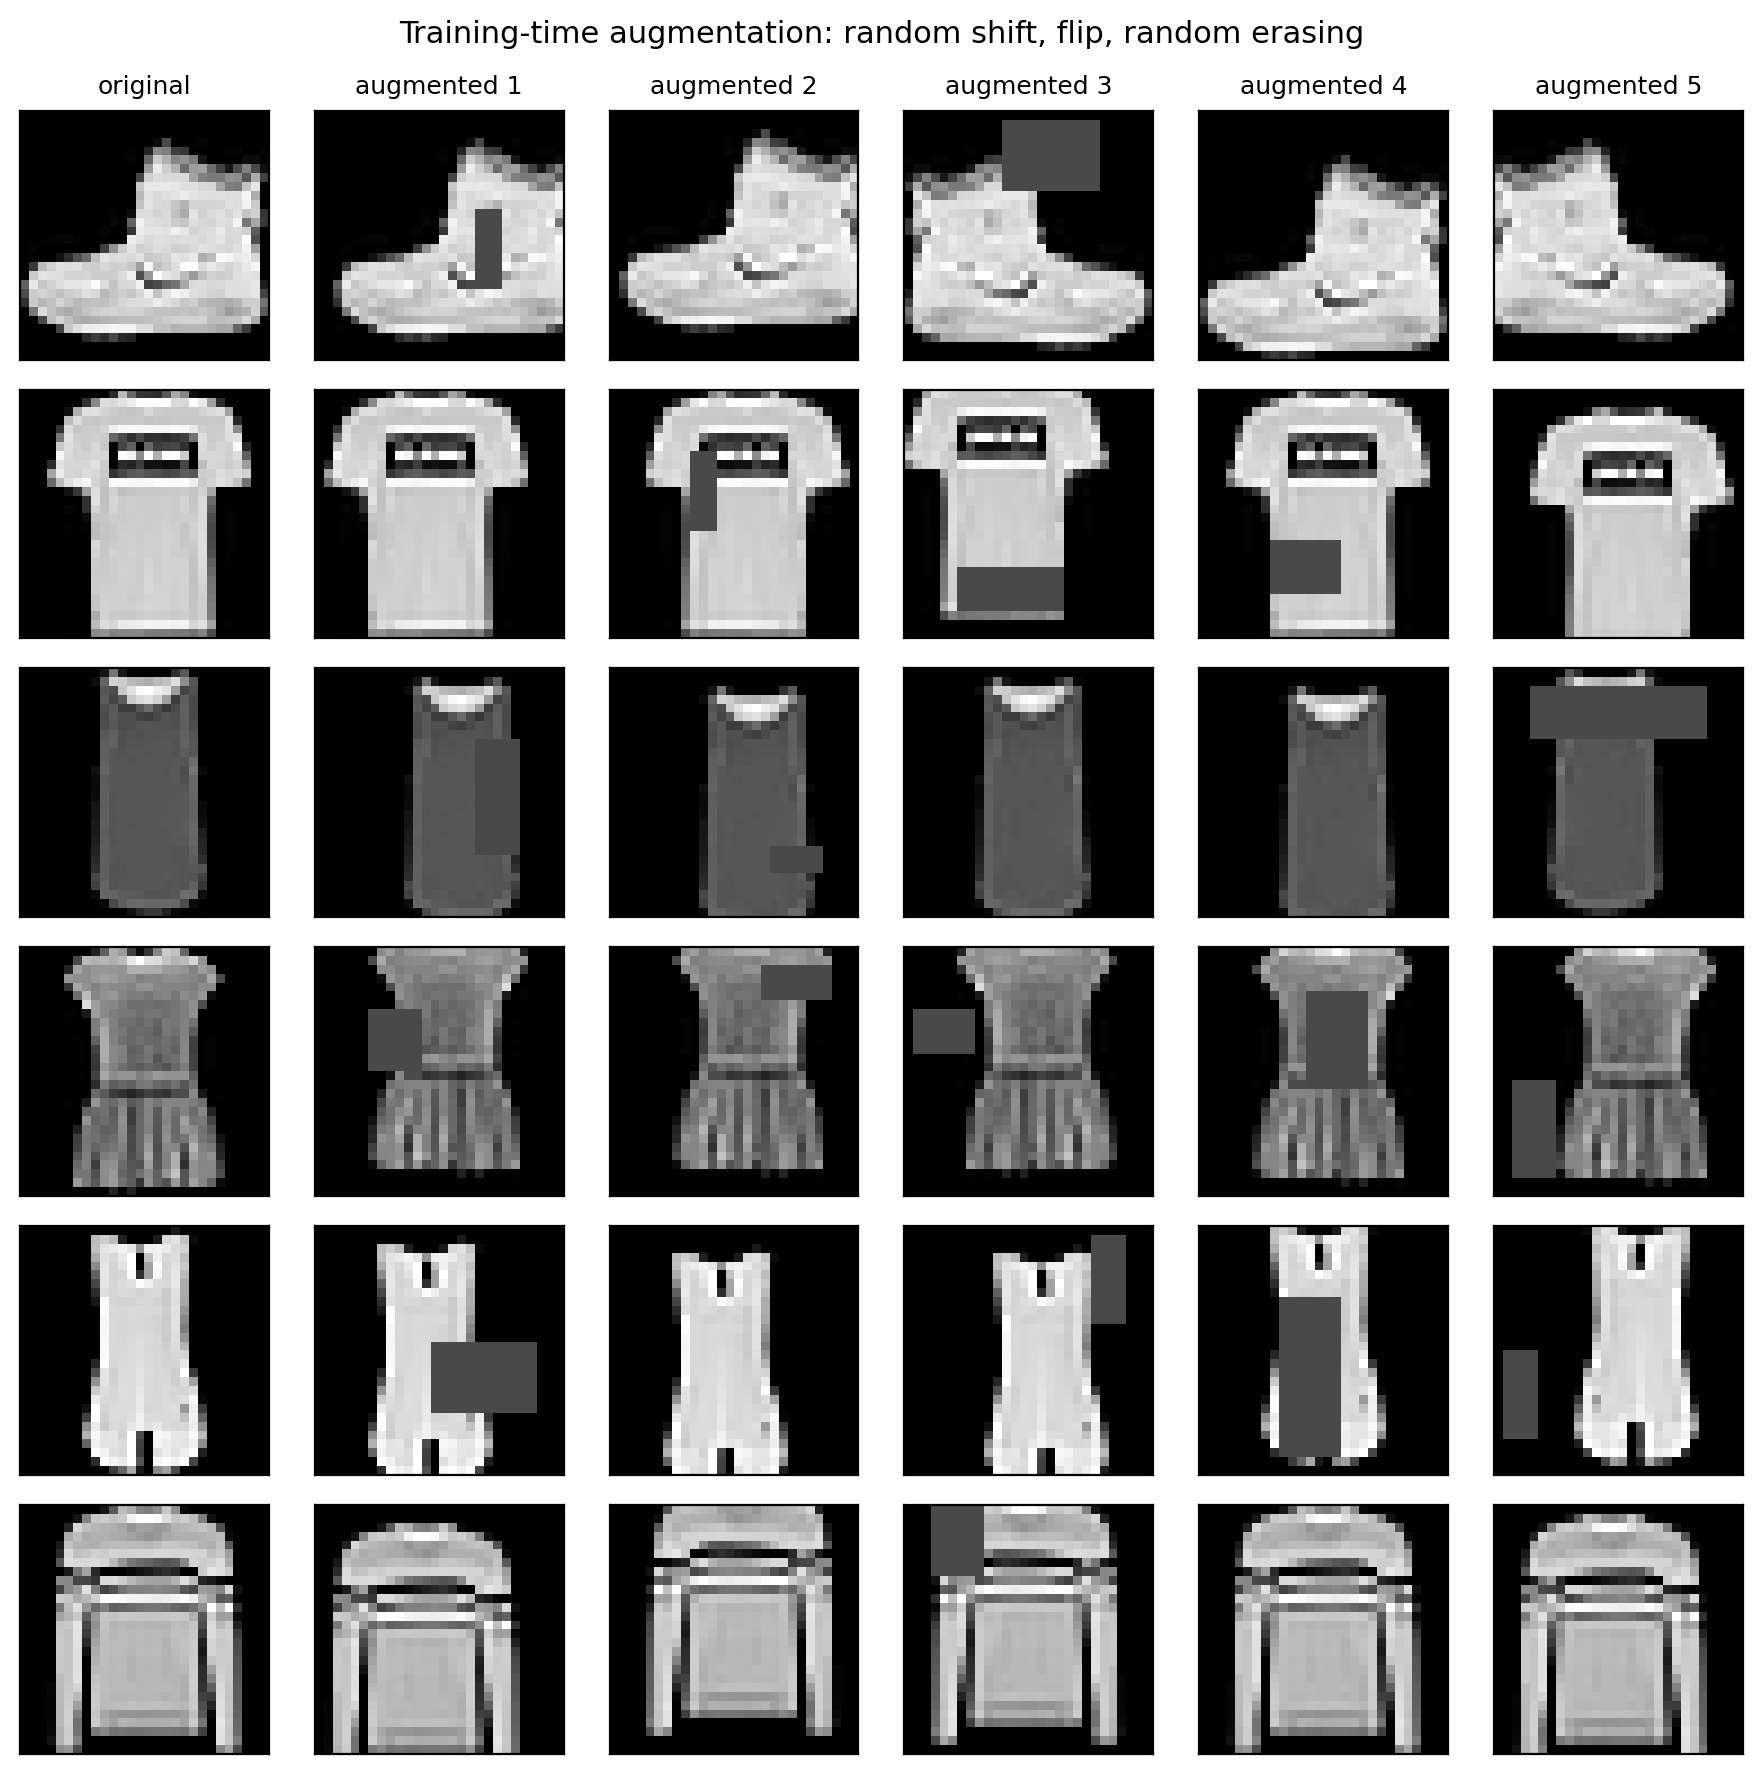
\includegraphics[width=\columnwidth]{augmentation_examples.png}
\caption{Training images (left column) and five augmented versions of each. Erasing is shown with a higher
probability than in training so that every row contains an example.}
\label{fig:p2aug}
\end{figure}

% Section owner: Manas (architecture and training engine)
\section{Architecture and Training}
\label{sec:p2arch}
\subsection{Limits of the Phase 1 CNN}
The Phase 1 CNN applies three blocks of one $3\times3$ convolution, ReLU and max-pooling, flattens the
$128\times3\times3$ output and classifies with two dense layers. Three properties limit it
(Table~\ref{tab:p2arch}). First, \DenseSharePone\% of its \ParamsPone{} parameters sit in dense layers, which do
not share weights across positions. Second, each resolution receives a single non-linear step, although the
confusable classes differ in small local patterns such as collars, plackets and sleeve length. Third, a unit of its
last feature map sees only $\RFPone\times\RFPone$ of the $28\times28$ pixels.

\subsection{FashionNet}
The Phase 2 family consists of a stem (one $3\times3$ convolution with 32 channels, batch normalisation, ReLU),
three stages of widths 32, 64 and 128 at resolutions 28, 14 and 7 separated by $2\times2$ max-pooling, global
average pooling, dropout and one linear layer. A stage contains $b$ blocks; a block computes
\begin{align}
F(x) &= \mathrm{BN}\bigl(\mathrm{conv}(\mathrm{ReLU}(\mathrm{BN}(\mathrm{conv}(x))))\bigr), \nonumber\\
y &= \mathrm{ReLU}\bigl(F(x) + s(x)\bigr),
\label{eq:p2block}
\end{align}
where $s$ is the identity, or a $1\times1$ convolution with batch normalisation when the number of channels
changes~\cite{he2016deep}. Since $\partial y/\partial x$ contains the identity term from $s$, the gradient reaches
early layers without passing through every convolution. Two stacked $3\times3$ convolutions cover a $5\times5$
region with 18 instead of 25 weights per channel pair~\cite{simonyan2015very}. Global average
pooling~\cite{lin2014network} replaces the $1152\rightarrow128$ dense layer; its 128 outputs are the embedding used
by the hybrid models. No pooling follows the last stage, because $7\times7$ cannot be halved without discarding a
row and a column.

Three switches turn the family into an experiment: \emph{residual} (remove $s$), \emph{batch normalisation}
(replace it by the identity and give the convolutions a bias), and the number of blocks per stage. The base model
uses $b=1$ (7 convolution layers, \ParamsBase{} parameters, receptive field \RFBase{} pixels); the deeper variant
uses $b=2$ (13 layers, \ParamsDeeper{} parameters).

% Generated by report/build_phase2_report_assets.py. Do not edit by hand.
\begin{table*}[t]
\centering
\caption{Architecture variants. Dense share is the fraction of parameters in fully connected layers; the receptive field is that of the last feature map. Validation macro-F1 is the mean $\pm$ standard deviation over three seeds.}
\label{tab:p2arch}
\footnotesize
\begin{tabular}{lrrrrr}
\toprule
Model & 3$\times$3 conv layers & Parameters & Dense share & Receptive field & Val macro-F1 \\
\midrule
Phase 1 CNN & 3 & 241,546 & 61.6\% & 22 px & 0.9343 $\pm$ 0.0023 \\
FashionNet, no shortcut & 7 & 297,450 & 0.4\% & 34 px & 0.9510 $\pm$ 0.0024 \\
FashionNet base & 7 & 308,074 & 0.4\% & 34 px & 0.9523 $\pm$ 0.0007 \\
FashionNet deeper (final) & 13 & 696,042 & 0.2\% & 62 px & 0.9557 $\pm$ 0.0010 \\
FashionNet narrow & 7 & 77,754 & 0.8\% & 34 px & 0.9413 $\pm$ 0.0014 \\
FashionNet, no BatchNorm & 7 & 307,402 & 0.4\% & 34 px & 0.9453 $\pm$ 0.0050 \\
\bottomrule
\end{tabular}
\end{table*}


\subsection{Training recipe}
The Phase 1 recipe is Adam with a constant learning rate of $10^{-3}$, no augmentation and early stopping with
patience 5. The Phase 2 recipe, fixed before any run, is AdamW~\cite{loshchilov2019decoupled} with learning rate
$2\times10^{-3}$ and weight decay $10^{-2}$ (not applied to biases and batch-normalisation parameters), one epoch
of linear warm-up followed by cosine decay to zero over 30 epochs~\cite{loshchilov2017sgdr}, batch size 128, label
smoothing 0.1, dropout 0.3 before the classifier, and the augmentation of Section~\ref{sec:p2data}. Early stopping
monitors the validation cross-entropy without label smoothing (patience 8) and the best weights are restored. On
the GPU the forward pass uses mixed precision. The seed fixes the initial weights, the batch order and the
augmentation draws.

% Section owner: Tanish (ablation design and regularisation theory)
\section{Ablation Design}
\label{sec:p2abl}
\subsection{Roadmap}
A comparison of the Phase 1 CNN with the new network would mix two changes, the architecture and the recipe. The
roadmap separates them in four steps: (1)~Phase 1 CNN with the Phase 1 recipe; (2)~Phase 1 CNN with the Phase 2
recipe; (3)~FashionNet without shortcuts; (4)~FashionNet with shortcuts, the base model.

\subsection{One-factor ablations}
Thirteen configurations change exactly one factor of the base (Table~\ref{tab:p2abl}); a unit test rejects a
configuration that differs from the base in more than its declared factor. Two couplings are declared: SGD uses its
own learning rate (0.05) and weight decay ($5\times10^{-4}$), and the constant schedule has no warm-up. Every
configuration is trained with seeds 42, 43 and 44. We report the paired difference in validation macro-F1 per
seed, variant minus base, because runs with the same seed share initial weights and batch order. A one-factor
design does not measure interactions between factors.

\subsection{What each regulariser is expected to do}
Regularisation trades a small increase in bias for a decrease in variance. We measure variance directly as the
generalisation gap, the training accuracy in evaluation mode minus the validation accuracy.

\emph{Dropout} sets each pooled feature to zero with probability $p$ during training, so the classifier cannot
depend on a single feature~\cite{srivastava2014dropout}. \emph{Decoupled weight decay} multiplies the weights by
$(1-\eta\lambda)$ at each step; because batch normalisation removes the scale of the preceding weights, its main
effect in a normalised network is to keep the effective learning rate from shrinking. \emph{Label smoothing} with
$\varepsilon=0.1$ sets the target of the true class to $1-\varepsilon+\varepsilon/K=0.91$ and of the other classes
to $\varepsilon/K=0.01$; cross-entropy with one-hot targets is minimised only by unbounded logits, and smoothing
bounds the optimal logit gap. \emph{Augmentation} adds invariances instead of restricting weights.
\emph{Cosine decay} reduces the gradient noise near the end of training, which a constant learning rate keeps at
a fixed level.

% Section owner: Anant (hybrid ML + DL)
\section{Hybrid Models}
\label{sec:p2hybrid}
\subsection{Motivation}
Phase 1 treated handcrafted features and the CNN as rivals. The two descriptions are built differently: HOG is a
fixed function of local gradient orientation, the CNN embedding is learned from the labels. If the models fail on
different images, a combination can in principle beat both. The hybrid tests whether a classical classifier can use
this.

\subsection{Models}
All classical heads are RBF-SVMs, the best classical model of Phase 1.
\begin{itemize}
\item \textbf{H0}: PCA-reduced HOG $\rightarrow$ SVM. Control with handcrafted features only.
\item \textbf{H1}: CNN embedding $\rightarrow$ SVM. Control with learned features and a classical classifier.
\item \textbf{H2}: [embedding, $\alpha\,\cdot$ PCA-HOG] $\rightarrow$ SVM. Feature-level fusion.
\item \textbf{H3}: the CNN decides when its largest softmax probability is at least $\tau$; otherwise H2 decides.
\end{itemize}
The controls make the claim falsifiable. If H2 exceeds the CNN but equals H1, the gain comes from the SVM head and
not from HOG; only H2 above H1 supports complementary information.

\subsection{Fusion vector}
The 128 embedding dimensions are standardised. The 6{,}084 HOG dimensions are reduced by PCA with whitening, so that
both blocks have unit variance per dimension. For two images $a$ and $b$ the RBF kernel then depends on
\begin{equation}
\|z_a-z_b\|^2=\|e_a-e_b\|^2+\alpha^2\|h_a-h_b\|^2,
\end{equation}
so $\alpha$ sets the weight of the handcrafted block. $C\in\{1,10\}$, the number of HOG components
$\in\{64,128\}$ and $\alpha\in\{0.5,1,2\}$ are chosen on validation with an SVM fitted on a stratified
10{,}000-image training subset, as in Phase 1; the final SVM is fitted on all 54{,}000 training images.
Hyper-parameters and $\tau$ are chosen with seed 42 and re-used for the other seeds. The scaler, the PCA (fitted on
a 20{,}000-image training subset) and the SVM never see validation or test images.

\subsection{Limitation}
The CNN was trained on the same images whose embeddings train the SVM, so training embeddings are cleaner than
embeddings of new images. Out-of-fold embeddings would remove this at several times the training cost; we keep the
simple version and judge it on validation and test.

% Section owner: Puneet (protocol) and Rohan (evaluation metrics)
\section{Protocol and Evaluation}
\label{sec:p2protocol}
\textbf{Selection.} All choices use validation data only. The final deep model is the configuration with the
highest mean validation macro-F1 over the three seeds (ties: accuracy, then fewer parameters); this rule is
implemented in code and was fixed before the runs.

\textbf{Freeze and test gate.} After selection and hybrid tuning, one file records the selected configuration,
the hybrid hyper-parameters, $\tau$, both recipes, the split hash and the list of \NGateModels{} models allowed on
the test set: for each seed the re-trained Phase 1 CNN, the final deep model, H1, H2 and H3, and H0. The test
set is loaded inside the gate, which refuses to run without the freeze file, with an existing flag file, or when
the evaluated models differ from the frozen list. The gate ran once on all 10{,}000 test images.

\textbf{Test-set reuse.} The same test images were evaluated once at the Phase 1 gate, and the Phase 1 error
analysis motivated Phase 2. Phase 2 test numbers are therefore slightly optimistic as estimates for new data.
Comparisons between Phase 2 models remain fair because all of them were selected on validation only.

\textbf{Two kinds of uncertainty.} Training randomness is reported as mean $\pm$ sample standard deviation over
three seeds. Test-set sampling is reported as a 95\% bootstrap interval (1{,}000 resamples) for seed 42. Pairs of
models are compared with McNemar's test on seed 42, Bonferroni-corrected for \NComparisons{} planned comparisons.
With three seeds the standard deviation is itself uncertain, so we use it descriptively.

\textbf{Further measurements.} Per-class recall; in-group confusion, the share of T-shirt, Pullover, Coat and
Shirt images assigned to another class of that group; the expected calibration error with 15 confidence
bins~\cite{guo2017calibration}; accuracy under five corruptions on a stratified subset of 2{,}000 test images; and
parameter counts and inference time.

\textbf{Compute.} All \NRuns{} runs were trained on one Tesla T4 GPU in \TrainMinutesTotal{} minutes of training
time in total (about \TrainSecondsDeeper{}~s per run for the final architecture and \TrainSecondsPone{}~s for the
Phase 1 CNN). Runs are stored individually and can be resumed.

% Section owners: Rohan (test analysis, statistics, calibration), Tanish (ablations), Anant (hybrid),
%                 Akhil (robustness), Manas (architecture and cost)
\section{Results}
\label{sec:p2results}
\subsection{Roadmap: recipe versus architecture}
Fig.~\ref{fig:p2roadmap} shows the four roadmap steps on validation data. Re-trained with three seeds, the Phase 1
CNN reaches \ValPoneRecipeOne{} $\pm$ \ValPoneRecipeOneStd{} macro-F1. Giving the same network the Phase 2 recipe
changes this by \RecipeOnPoneDelta{} percentage points (pp), a decrease in \RecipeOnPoneAllNegative{} seeds. Its
training accuracy falls to \ValPoneRecipeTwoTrainAcc{} and its generalisation gap to \ValPoneRecipeTwoGap{}~pp: the
small network has no over-fitting left to remove, and stronger regularisation only makes the training task harder.
Under the same recipe, replacing the architecture adds \ArchGainSameRecipe{}~pp. The gain of Phase 2 therefore
comes from the architecture, and the recipe pays off only once the model has the capacity to use it. Adding
shortcuts to the seven-layer network changes macro-F1 by $\ShortcutGain$~pp, with seeds disagreeing on the sign.

\begin{figure}[t]
\centering
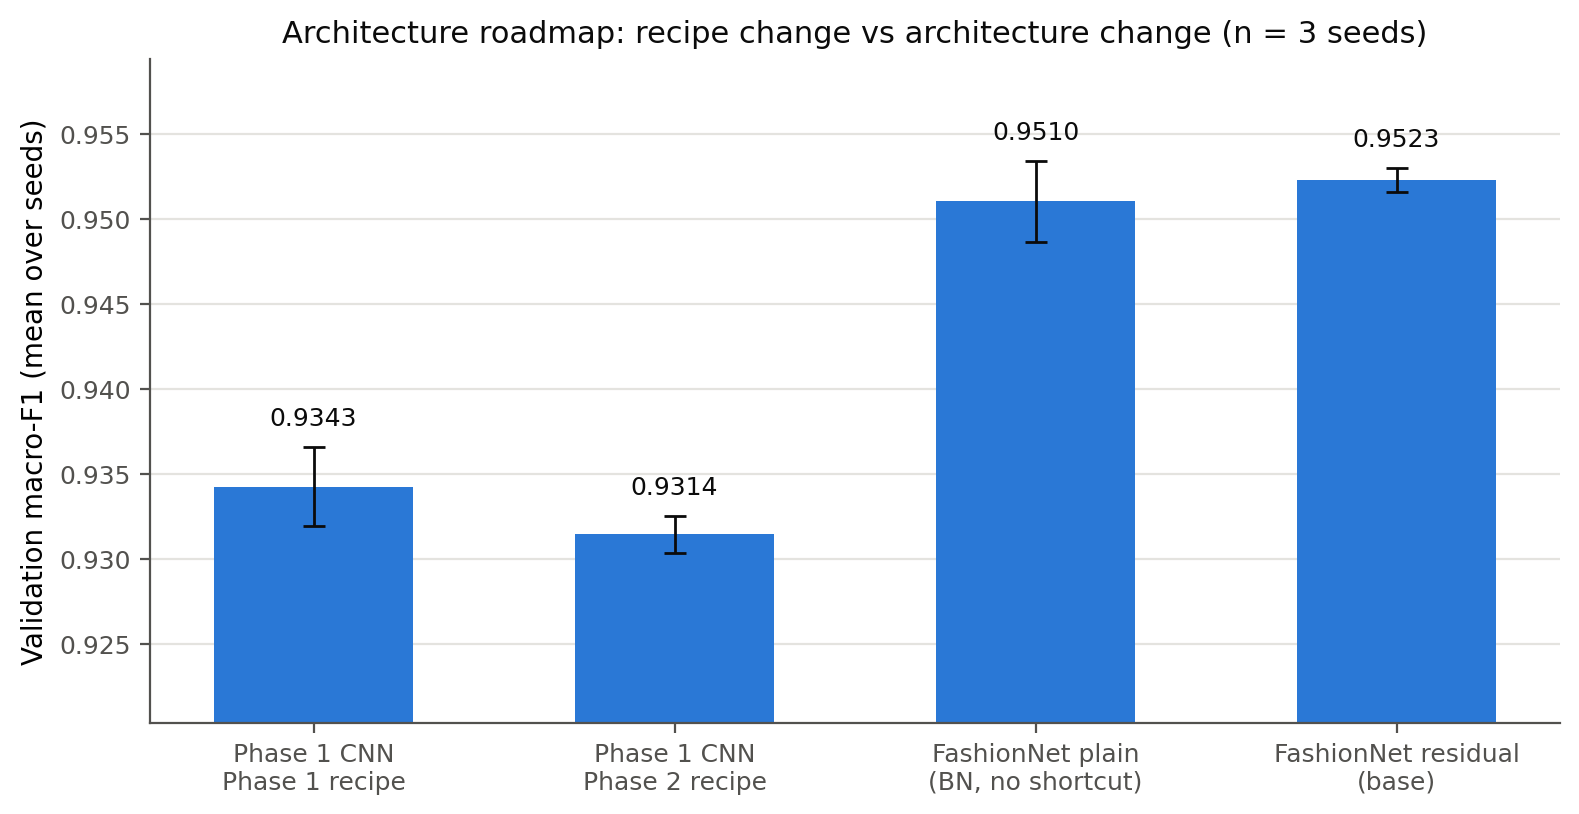
\includegraphics[width=\columnwidth]{architecture_roadmap.png}
\caption{Architecture roadmap on validation data (mean over three seeds, whiskers $\pm1$ standard deviation).}
\label{fig:p2roadmap}
\end{figure}

% Generated by report/build_phase2_report_assets.py. Do not edit by hand.
\begin{table*}[t]
\centering
\caption{Validation results of all 16 configurations (three seeds each). $\Delta$ is the paired change in macro-F1 relative to the base in percentage points (variant minus base, same seed); a negative value means that the factor present in the base helps. Gap is training accuracy minus validation accuracy.}
\label{tab:p2abl}
\footnotesize
\begin{tabular}{llrrrrrr}
\toprule
Group & Change relative to base & Val macro-F1 & $\Delta$ (pp) & Range over seeds (pp) & Seeds agree & Gap (pp) & Shirt recall \\
\midrule
roadmap & Phase 1 CNN, Phase 1 recipe & 0.9343 $\pm$ 0.0023 & -1.80 & -2.03 to -1.66 & yes & 2.74 & 0.796 \\
roadmap & Phase 1 CNN, Phase 2 recipe & 0.9314 $\pm$ 0.0011 & -2.09 & -2.18 to -2.03 & yes & 0.29 & 0.761 \\
\midrule
base & FashionNet base (reference) & 0.9523 $\pm$ 0.0007 & -- & -- & -- & 1.49 & 0.849 \\
\midrule
architecture & no residual shortcut & 0.9510 $\pm$ 0.0024 & -0.13 & -0.26 to +0.15 & no & 1.74 & 0.848 \\
architecture & no batch normalisation & 0.9453 $\pm$ 0.0050 & -0.70 & -1.27 to -0.30 & yes & 0.83 & 0.823 \\
architecture & 2 blocks per stage (13 conv layers) & 0.9557 $\pm$ 0.0010 & +0.34 & +0.24 to +0.45 & yes & 2.53 & 0.863 \\
architecture & widths 16/32/64 & 0.9413 $\pm$ 0.0014 & -1.10 & -1.19 to -0.97 & yes & 0.44 & 0.809 \\
\midrule
regularisation & dropout 0.0 (base 0.3) & 0.9525 $\pm$ 0.0026 & +0.02 & -0.20 to +0.26 & no & 1.68 & 0.851 \\
regularisation & dropout 0.5 & 0.9504 $\pm$ 0.0010 & -0.18 & -0.29 to -0.03 & yes & 1.63 & 0.848 \\
regularisation & no weight decay & 0.9513 $\pm$ 0.0023 & -0.10 & -0.28 to +0.03 & no & 1.65 & 0.848 \\
regularisation & no label smoothing & 0.9494 $\pm$ 0.0019 & -0.29 & -0.46 to -0.17 & yes & 1.81 & 0.848 \\
\midrule
augmentation & no augmentation & 0.9451 $\pm$ 0.0041 & -0.72 & -1.04 to -0.28 & yes & 5.35 & 0.796 \\
augmentation & no horizontal flip & 0.9523 $\pm$ 0.0009 & +0.00 & -0.03 to +0.03 & no & 2.74 & 0.857 \\
augmentation & no random erasing & 0.9507 $\pm$ 0.0012 & -0.16 & -0.24 to -0.09 & yes & 2.10 & 0.844 \\
\midrule
optimisation & SGD + Nesterov momentum & 0.9514 $\pm$ 0.0019 & -0.09 & -0.25 to +0.05 & no & 1.42 & 0.846 \\
optimisation & constant learning rate & 0.9455 $\pm$ 0.0028 & -0.68 & -0.94 to -0.46 & yes & 1.18 & 0.824 \\
\bottomrule
\end{tabular}
\end{table*}


\begin{figure*}[t]
\centering
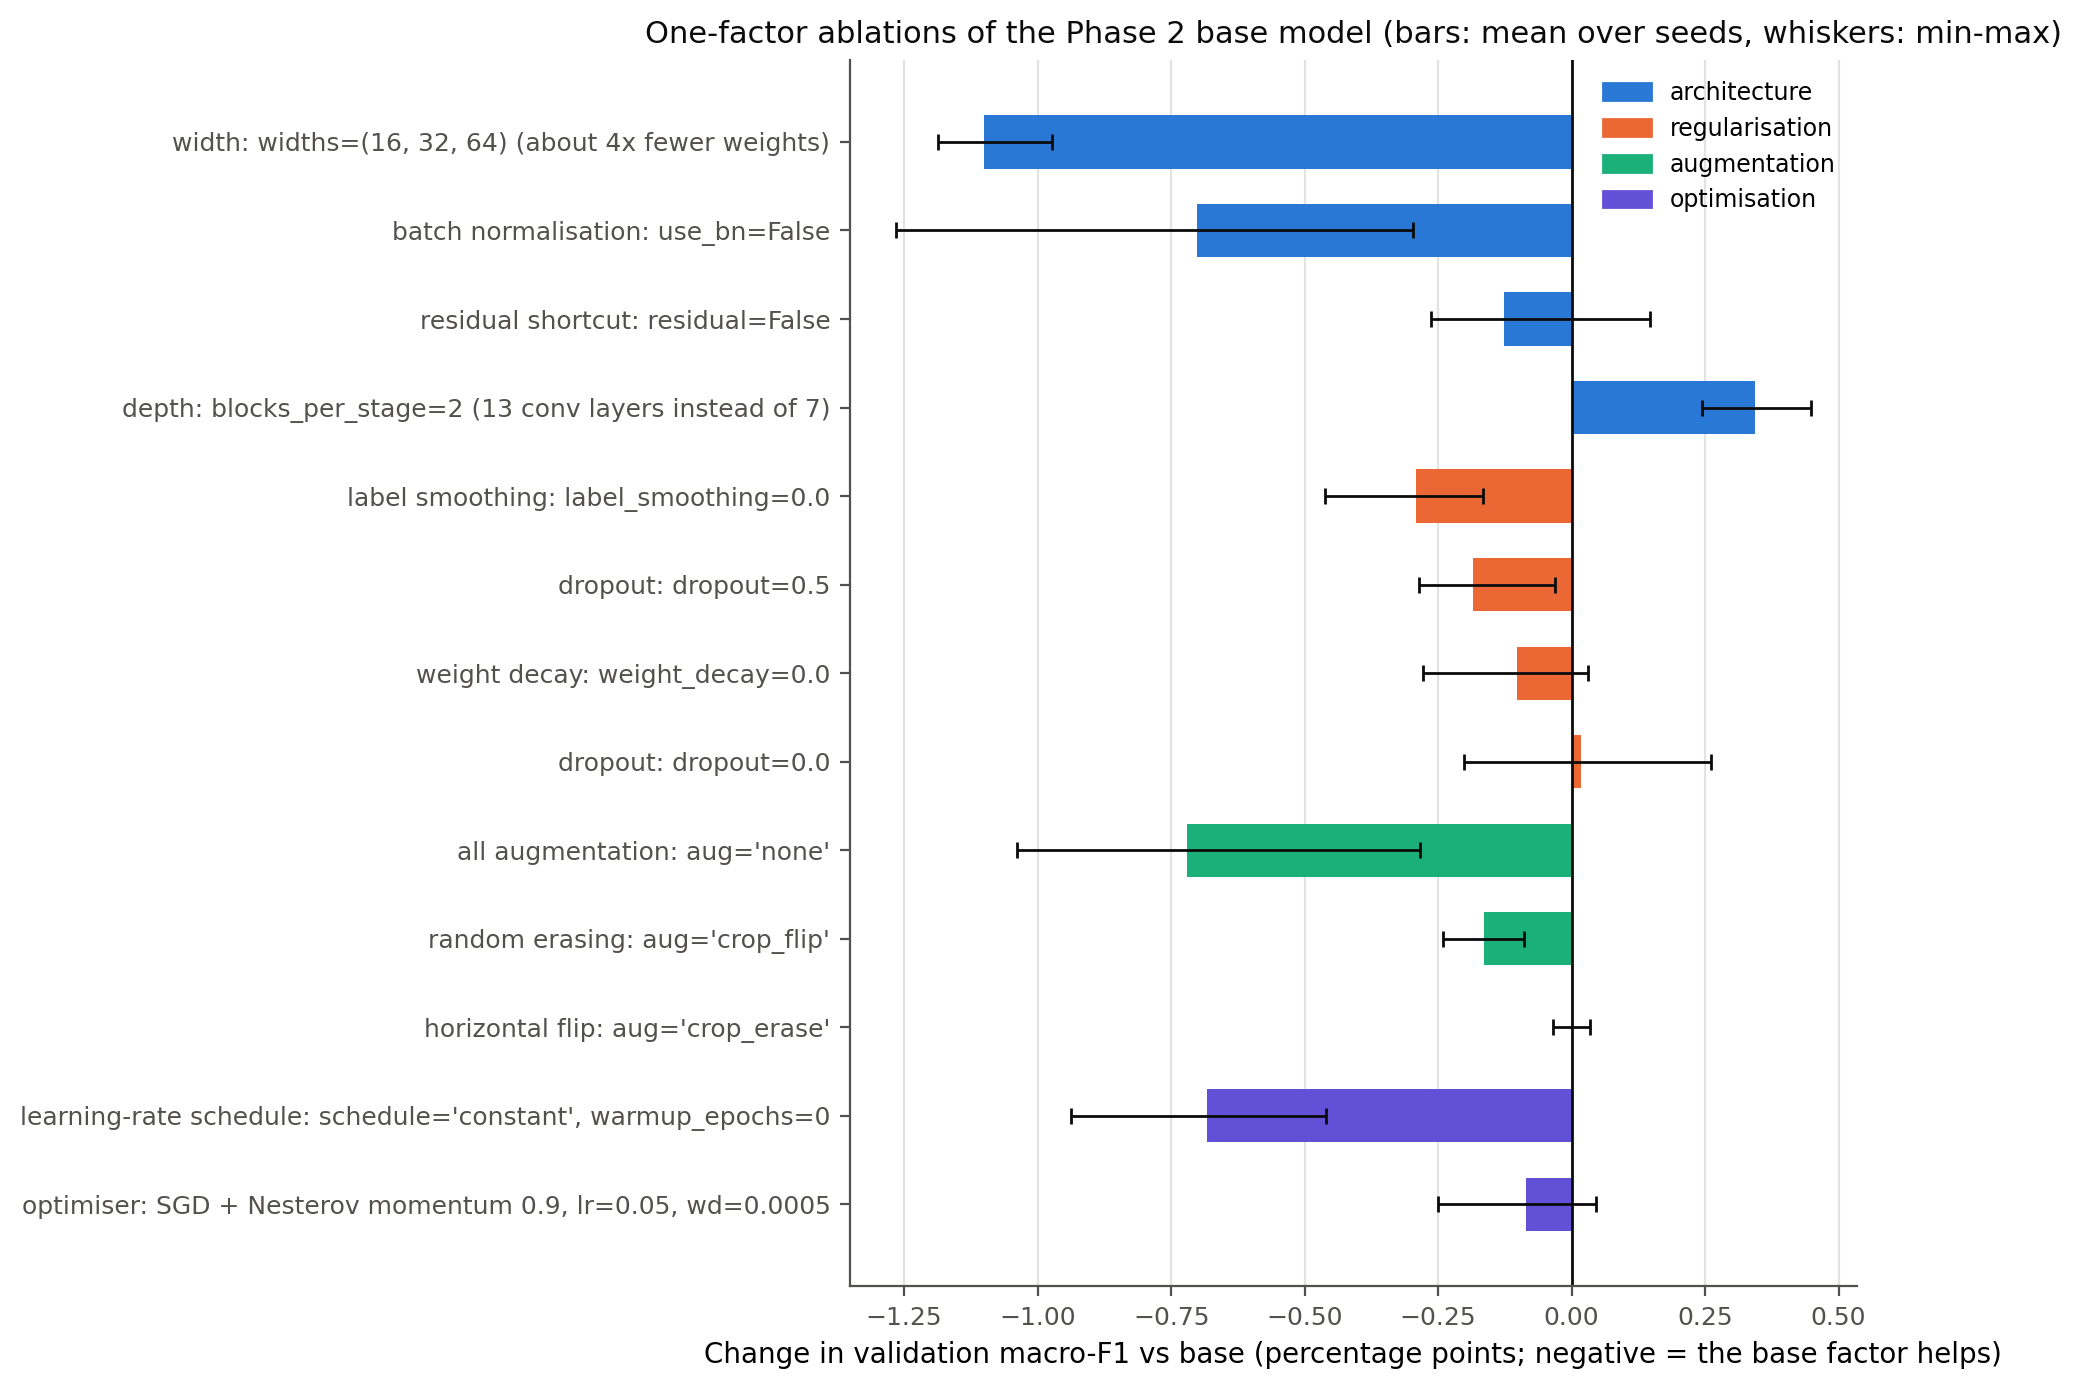
\includegraphics[width=0.8\textwidth]{ablation_deltas.png}
\caption{One-factor ablations: paired change in validation macro-F1 relative to the base model.}
\label{fig:p2abl}
\end{figure*}

\subsection{Ablations}
Table~\ref{tab:p2abl} and Fig.~\ref{fig:p2abl} give all configurations.

\emph{Capacity.} Reducing the widths to 16/32/64 (\ParamsNarrow{} parameters) costs \DeltaNarrow{}~pp, the largest
effect in the study. Doubling the depth gains \DeltaDeeper{}~pp in every seed and has the highest mean validation
macro-F1 (\ValDeeper{} $\pm$ \ValDeeperStd); by the selection rule it is the final deep model.

\emph{Batch normalisation.} Removing it costs \DeltaNoBN{}~pp and raises the standard deviation over seeds from
\BaseStdPP{} to \NoBNStd{}~pp: the network is both less accurate and less stable at the fixed learning rate.

\emph{Augmentation.} Without augmentation the network reaches \ValNoAugTrainAcc{} training accuracy, a gap of
\ValNoAugGap{}~pp, and loses \DeltaNoAug{}~pp (Fig.~\ref{fig:p2gap}). Random erasing contributes
\DeltaNoErase{}~pp when removed, consistently. Removing the horizontal flip changes nothing ($\DeltaNoFlip$~pp), as
expected for near-symmetric garments.

\emph{Other regularisers.} Removing label smoothing costs \DeltaNoLS{}~pp in every seed. Dropout 0.5 instead of 0.3
costs \DeltaDropHalf{}~pp. Removing dropout ($\DeltaDropZero$~pp) or weight decay ($\DeltaNoWD$~pp) has no
measurable effect: the seeds disagree on the sign.

\emph{Optimisation.} A constant learning rate costs \DeltaConstLR{}~pp. SGD with Nesterov momentum is within
noise of AdamW ($\DeltaSGD$~pp, inconsistent sign), so the result does not depend on the adaptive optimiser.

\begin{figure}[t]
\centering
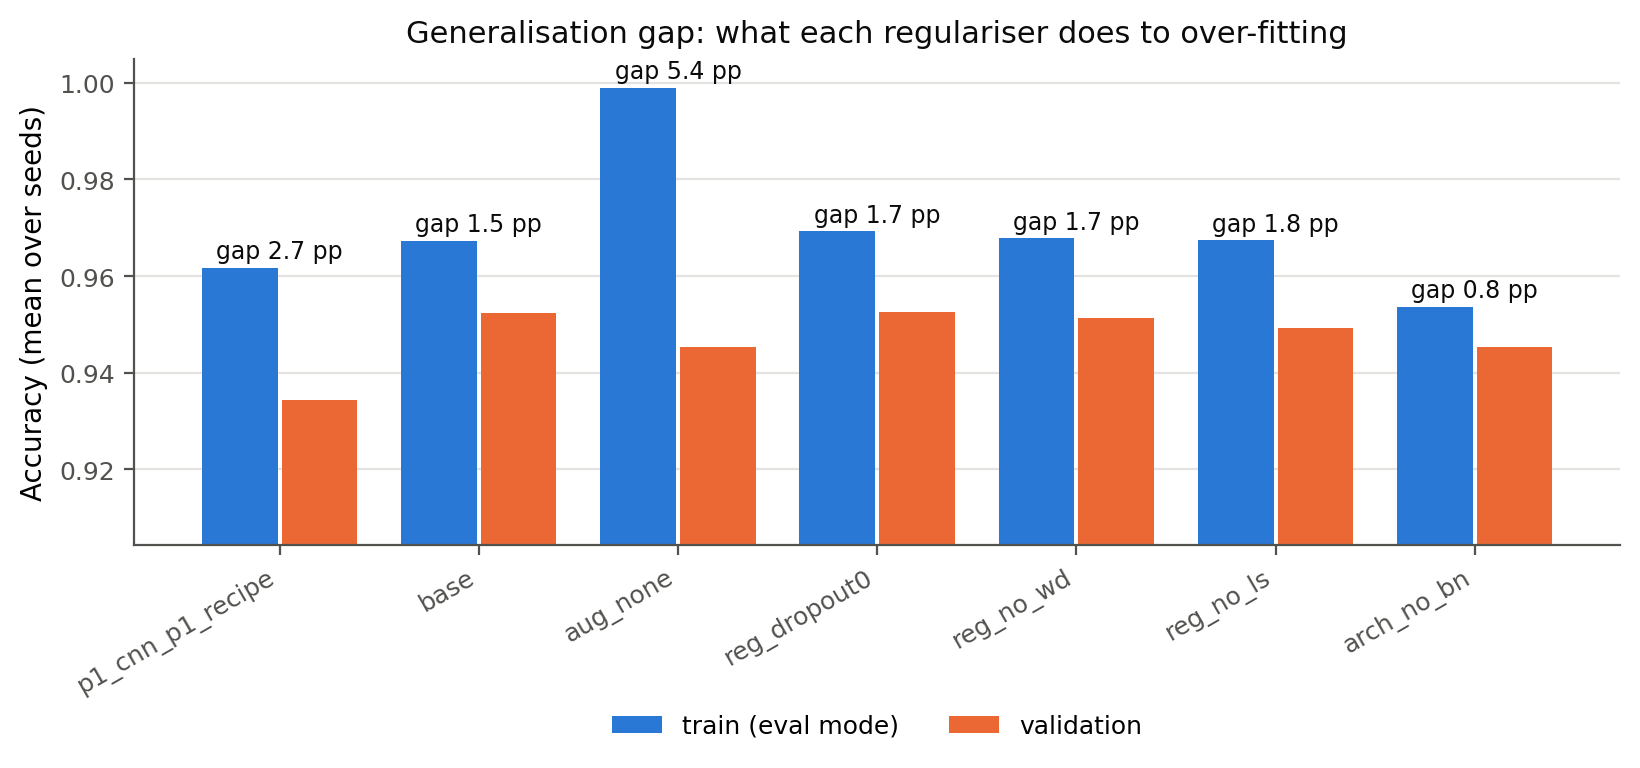
\includegraphics[width=\columnwidth]{generalisation_gap.png}
\caption{Training accuracy (evaluation mode) and validation accuracy for selected configurations.}
\label{fig:p2gap}
\end{figure}

\begin{figure*}[t]
\centering
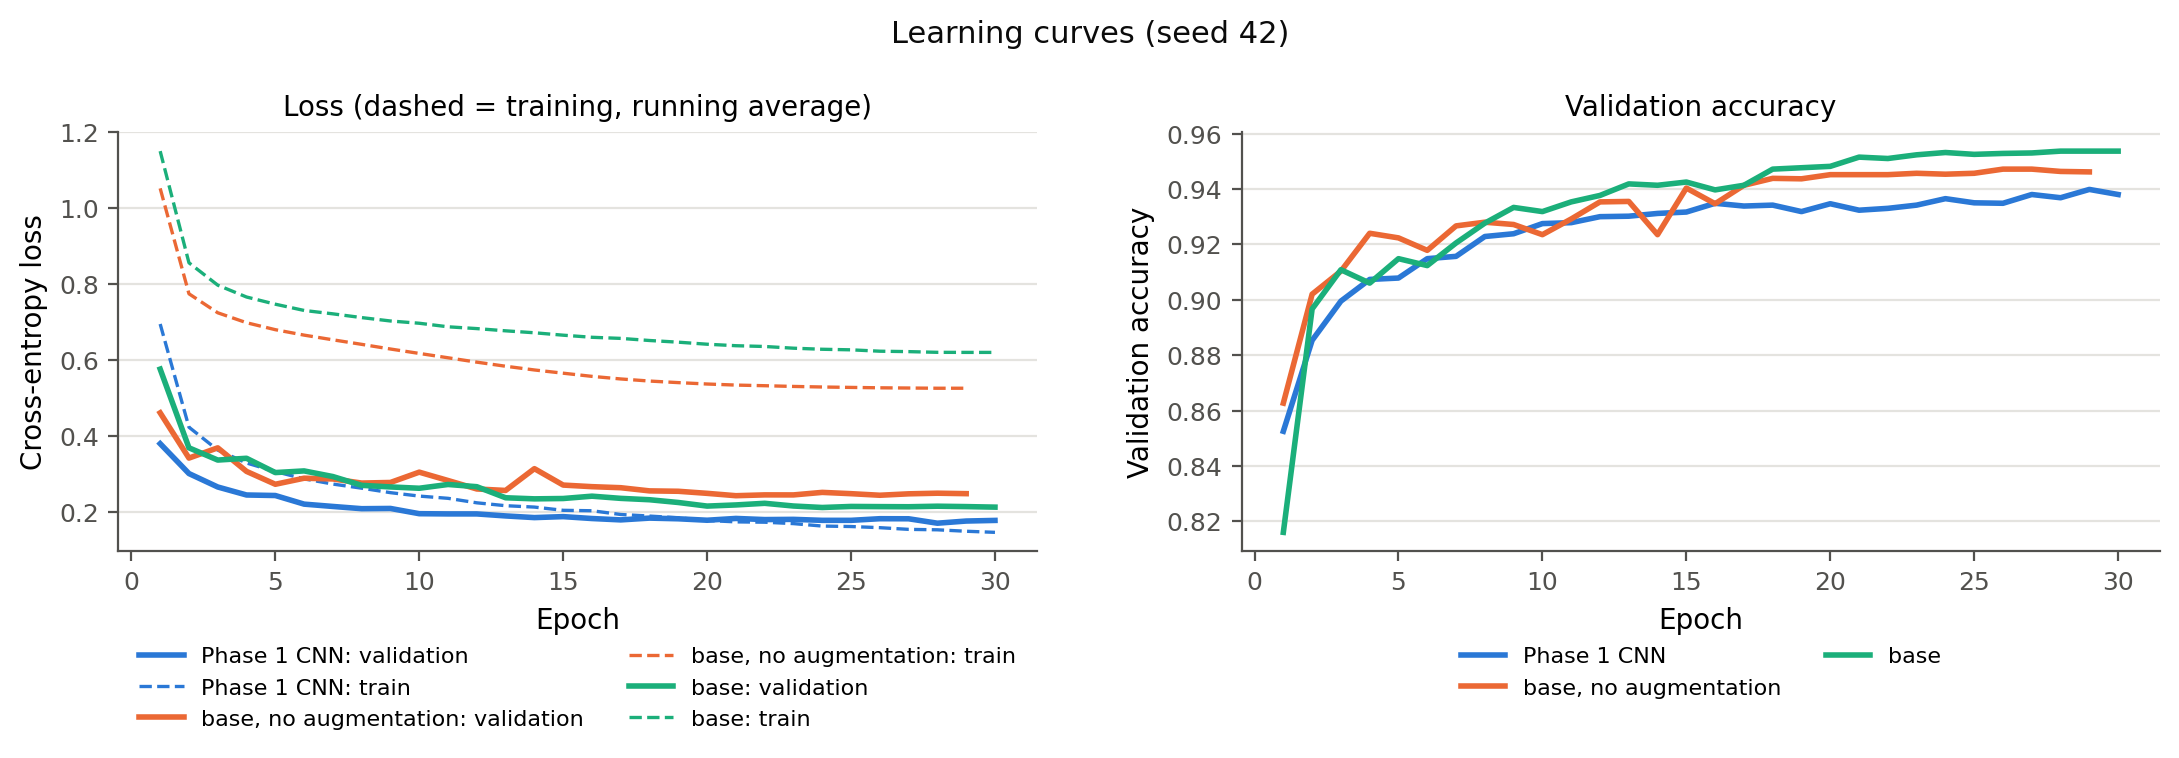
\includegraphics[width=0.85\textwidth]{learning_curves.png}
\caption{Learning curves for seed 42. Training loss is higher than validation loss for the base model because it
is measured with augmentation, dropout and label smoothing.}
\label{fig:p2curves}
\end{figure*}

\subsection{Test results of the final deep model}
Table~\ref{tab:p2test} reports the frozen models. The final deep model reaches \TestFinal{} $\pm$ \TestFinalStd{}
accuracy; the re-trained Phase 1 CNN reaches \TestPone{} $\pm$ \TestPoneStd, a range that contains the single
Phase 1 result of \PhaseOneCnnAcc. The difference is \TestGainFinalVsPone{}~pp, more than six times the larger
of the two standard deviations. The mean number of errors falls from \ErrorsPoneMean{} to \ErrorsFinalMean{}
(\ErrorReduction\% fewer). For seed 42 the final model is right on \McFinalOnly{} images on which the Phase 1 CNN
is wrong and wrong on \McPoneOnly{} on which it is right ($p<10^{-4}$, Table~\ref{tab:p2mcnemar}).

The gain is concentrated where Phase 1 was weakest (Fig.~\ref{fig:p2recall}). Mean Shirt recall rises from
\TestPoneShirt{} to \TestFinalShirt, and in-group confusion among the four upper-body classes falls from
\TestPoneInGroup\% to \TestFinalInGroup\%. Shirt remains the hardest class; its most frequent error is still
T-shirt/top (Fig.~\ref{fig:p2cm}).

% Generated by report/build_phase2_report_assets.py. Do not edit by hand.
\begin{table*}[t]
\centering
\caption{Test results of the frozen Phase 2 models: mean $\pm$ standard deviation over three training seeds (H0 does not depend on the seed). The interval is a 95\% bootstrap interval over test images for seed 42. In-group confusion is the share of T-shirt, Pullover, Coat and Shirt images assigned to another class of that group.}
\label{tab:p2test}
\footnotesize
\begin{tabular}{lrrrrr}
\toprule
Model & Accuracy & Macro-F1 & 95\% CI (seed 42) & Shirt recall & In-group confusion \\
\midrule
H0: PCA-HOG + SVM (classical) & 0.9048 $\pm$ 0.0000 & 0.9047 $\pm$ 0.0000 & [0.8990, 0.9102] & 0.708 & 15.3\% \\
Phase 1 CNN, re-trained & 0.9252 $\pm$ 0.0034 & 0.9250 $\pm$ 0.0030 & [0.9231, 0.9332] & 0.757 & 12.2\% \\
Final deep model & 0.9488 $\pm$ 0.0015 & 0.9487 $\pm$ 0.0014 & [0.9445, 0.9532] & 0.834 & 8.5\% \\
H1: CNN embedding + SVM & 0.9495 $\pm$ 0.0009 & 0.9494 $\pm$ 0.0009 & [0.9454, 0.9540] & 0.833 & 8.4\% \\
H2: embedding + HOG fusion SVM & 0.9502 $\pm$ 0.0020 & 0.9501 $\pm$ 0.0020 & [0.9455, 0.9539] & 0.839 & 8.3\% \\
H3: confidence-gated cascade & 0.9502 $\pm$ 0.0021 & 0.9501 $\pm$ 0.0021 & [0.9455, 0.9539] & 0.839 & 8.3\% \\
\bottomrule
\end{tabular}
\end{table*}

% Generated by report/build_phase2_report_assets.py. Do not edit by hand.
\begin{table*}[t]
\centering
\caption{McNemar tests on the test set for seed 42 (A vs.\ B). The corrected $p$-value is Bonferroni-adjusted for 7 planned comparisons.}
\label{tab:p2mcnemar}
\footnotesize
\begin{tabular}{llrrrrr}
\toprule
Model A & Model B & Only A right & Only B right & $p$ & $p$ corrected & Significant \\
\midrule
Final deep model & Phase 1 CNN, re-trained & 367 & 158 & $<10^{-4}$ & $<10^{-4}$ & yes \\
H1 & Final deep model & 27 & 18 & 0.233 & 1.000 & no \\
H2 & Final deep model & 36 & 25 & 0.200 & 1.000 & no \\
H3 & Final deep model & 36 & 25 & 0.200 & 1.000 & no \\
H2 & H1 & 33 & 31 & 0.901 & 1.000 & no \\
Final deep model & Phase 1 CNN, original & 377 & 161 & $<10^{-4}$ & $<10^{-4}$ & yes \\
Final deep model & Phase 1 pixel SVM & 718 & 181 & $<10^{-4}$ & $<10^{-4}$ & yes \\
\bottomrule
\end{tabular}
\end{table*}


\begin{figure*}[t]
\centering
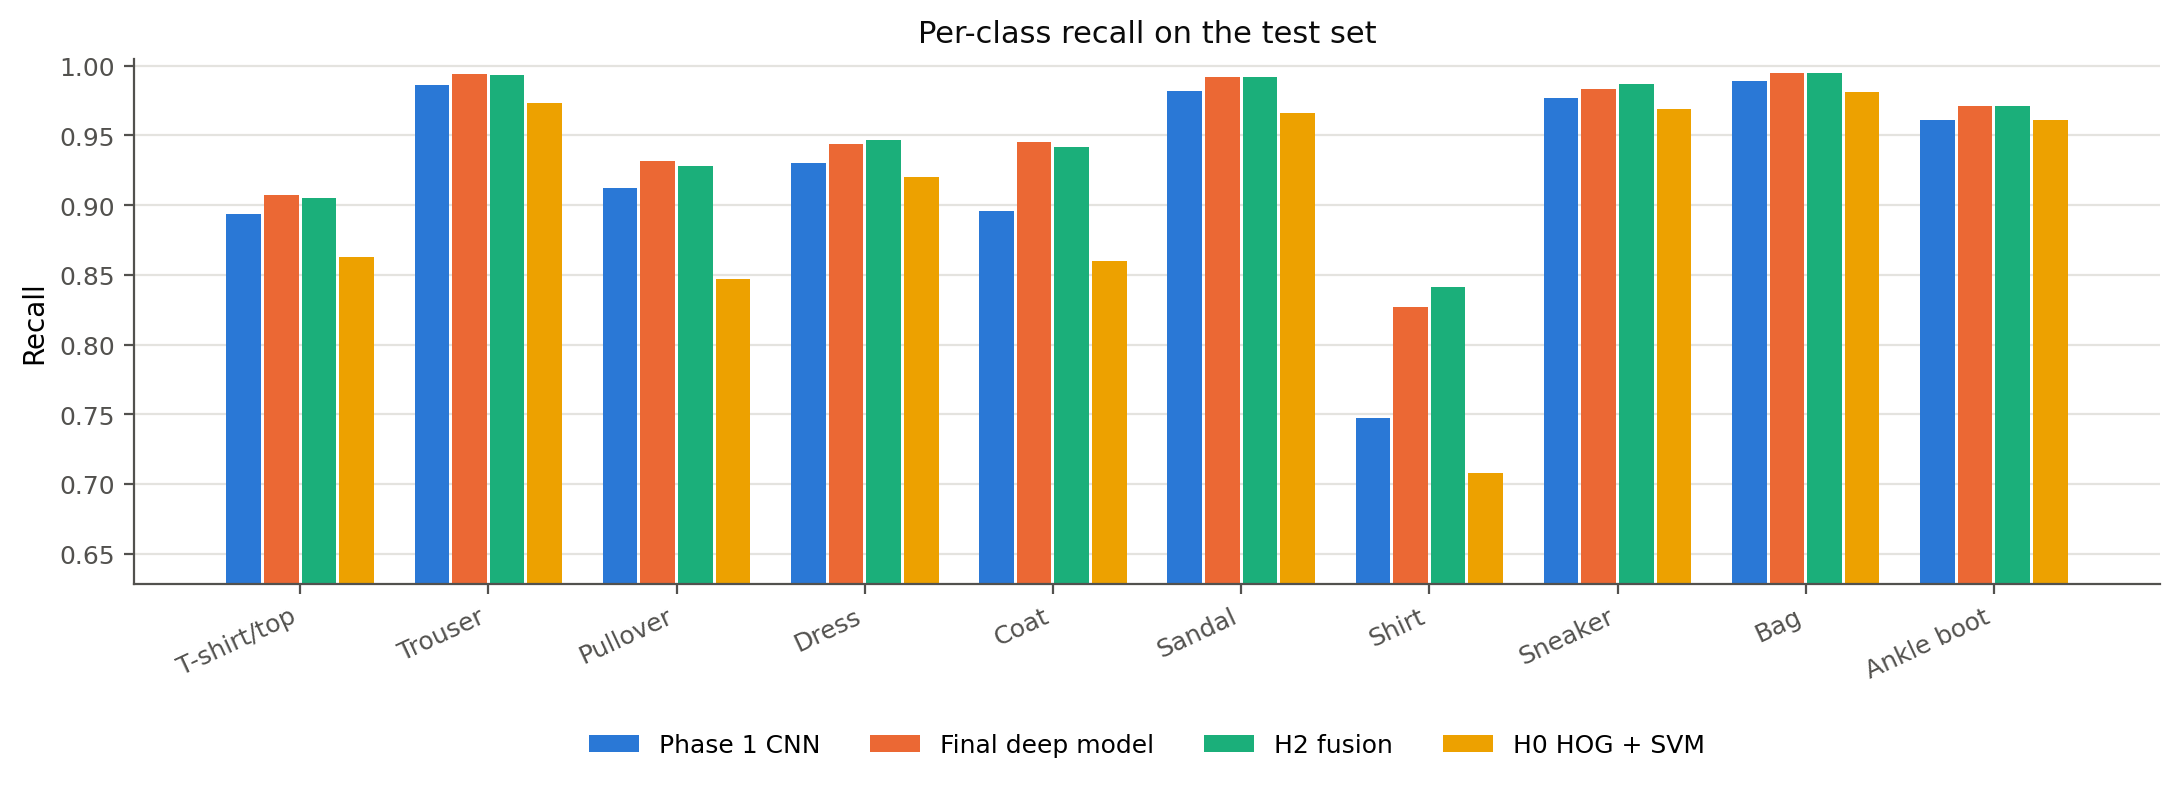
\includegraphics[width=0.85\textwidth]{per_class_recall_phase2.png}
\caption{Per-class recall on the test set (seed 42; Phase 1 CNN from the stored Phase 1 predictions).}
\label{fig:p2recall}
\end{figure*}

\begin{figure}[t]
\centering
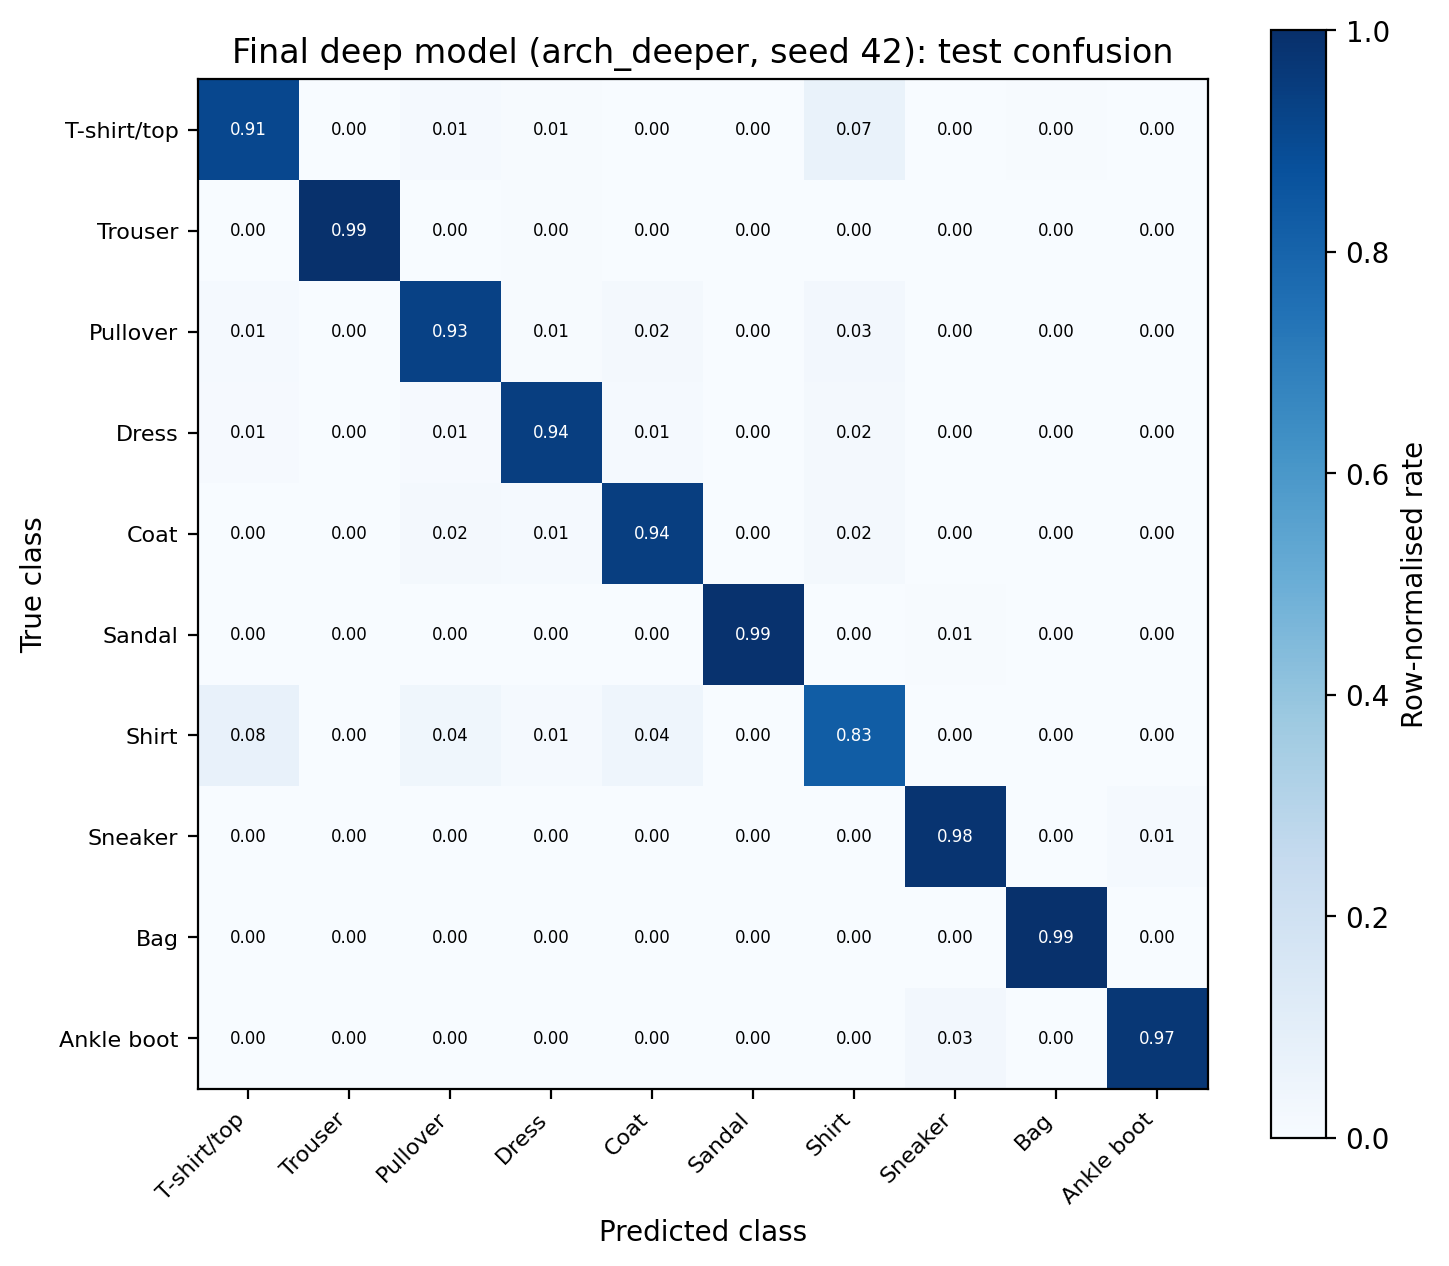
\includegraphics[width=\columnwidth]{cm_final_dl.png}
\caption{Row-normalised test confusion matrix of the final deep model (seed 42).}
\label{fig:p2cm}
\end{figure}

\subsection{Hybrid models}
\emph{Complementarity exists.} On the test set (seed 42) the handcrafted model H0 is correct on \CompHogFixes{}
of the \CompCnnErrors{} images that the deep model gets wrong (\CompHogFixShare\%). A selector that always
picked the correct model would reach \CompOracle. This is an upper bound that uses the true label.

\emph{The fusion gain is small and not significant.} H2 scores \TestHtwo{} $\pm$ \TestHtwoStd{}
(Table~\ref{tab:p2hybrid}). It is above the deep model in all three seeds, by \HtwoGain{}~pp on average
(\HtwoGainMin{} to \HtwoGainMax), and by \HtwoGainVal{}~pp on validation. This is the same size as the
seed-to-seed standard deviation. McNemar's test for seed 42 gives $p=\PHtwoVsFinal$ before correction: H2 fixes
\McHtwoOnly{} errors of the deep model and introduces \McFinalOnlyVsHtwo. The control H1 gains \HoneGain{}~pp, and
H2 against H1 gives $p=\PHtwoVsHone$. We conclude that the direction is consistent but the data do not show that
HOG adds to the embedding: most of the complementary images cannot be identified without the label.

\emph{The cascade keeps the accuracy at a fraction of the cost.} With $\tau=\Tau$ chosen on validation, H3
sends \RoutedTest\% of the test images to H2 and scores \TestHthree{} $\pm$ \TestHthreeStd, equal to H2. HOG
extraction and the SVM are needed for about one image in seventeen (Fig.~\ref{fig:p2cascade}).

\emph{A stronger classical baseline.} H0 reaches \TestHzero{} on the test set, above the \PhaseOneHogSvmAcc{} of
the Phase 1 HOG SVM, which had to be fitted on 11{,}770 images because of its 6{,}084 input dimensions. Reducing
HOG to 128 principal components (\PcaVar\% of the variance) made a fit on all 54{,}000 images feasible.

% Generated by report/build_phase2_report_assets.py. Do not edit by hand.
\begin{table}[t]
\centering
\caption{Test accuracy per training seed: final deep model and the hybrids built on it. The last column is H2 minus the deep model in percentage points.}
\label{tab:p2hybrid}
\footnotesize
\begin{tabular}{lrrrrr}
\toprule
Seed & Deep & H1 & H2 & H3 & H2 $-$ deep \\
\midrule
42 & 0.9490 & 0.9499 & 0.9501 & 0.9501 & +0.11 \\
43 & 0.9472 & 0.9485 & 0.9483 & 0.9482 & +0.11 \\
44 & 0.9501 & 0.9502 & 0.9523 & 0.9523 & +0.22 \\
\midrule
mean & 0.9488 & 0.9495 & 0.9502 & 0.9502 & +0.15 \\
\bottomrule
\end{tabular}
\end{table}


\begin{figure}[t]
\centering
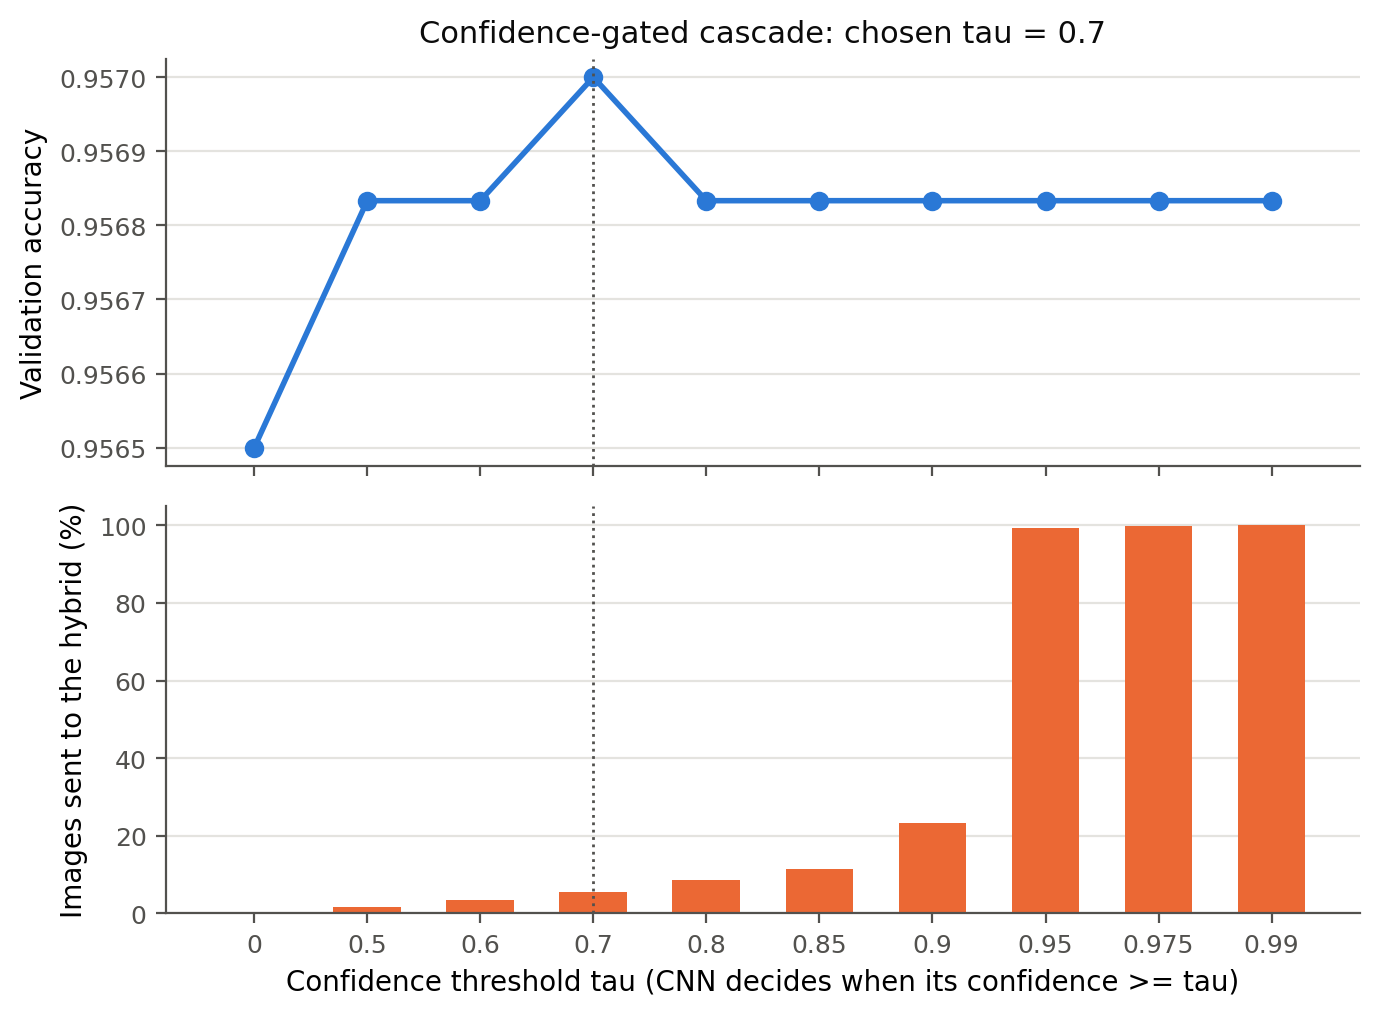
\includegraphics[width=0.9\columnwidth]{cascade_threshold.png}
\caption{Cascade threshold on validation data (seed 42): accuracy and share of images routed to H2.}
\label{fig:p2cascade}
\end{figure}

\subsection{Calibration}
The final model is under-confident: its mean confidence on the test set is \ConfFinalTest{} at \TestFinal{}
accuracy, and its expected calibration error is \EceFinalTest{} against \EcePoneTest{} for the Phase 1 CNN
(Table~\ref{tab:p2cal}). The ablation isolates the cause. On validation, the base model has an error of
\EceBaseVal{} with label smoothing and \EceNoLSVal{} without it (Fig.~\ref{fig:p2rel}). Label smoothing therefore
buys \GainLS{}~pp of macro-F1 at the price of calibration. The model without smoothing was
already well calibrated, so smoothing over-corrected. Confidence still ranks predictions, which is all the cascade
needs, but the probabilities should be rescaled before they are shown to a user.

% Generated by report/build_phase2_report_assets.py. Do not edit by hand.
\begin{table}[t]
\centering
\caption{Calibration: expected calibration error (15 bins), mean confidence and accuracy. Test rows are means over three seeds; validation rows are seed 42.}
\label{tab:p2cal}
\footnotesize
\begin{tabular}{llrrr}
\toprule
Model & Split & ECE & Confidence & Accuracy \\
\midrule
Phase 1 CNN & test & 0.013 & 0.935 & 0.925 \\
Final deep model & test & 0.067 & 0.886 & 0.949 \\
\midrule
Base, smoothing 0.1 & val & 0.083 & 0.870 & 0.953 \\
Base, no smoothing & val & 0.010 & 0.961 & 0.951 \\
\bottomrule
\end{tabular}
\end{table}


\begin{figure}[t]
\centering
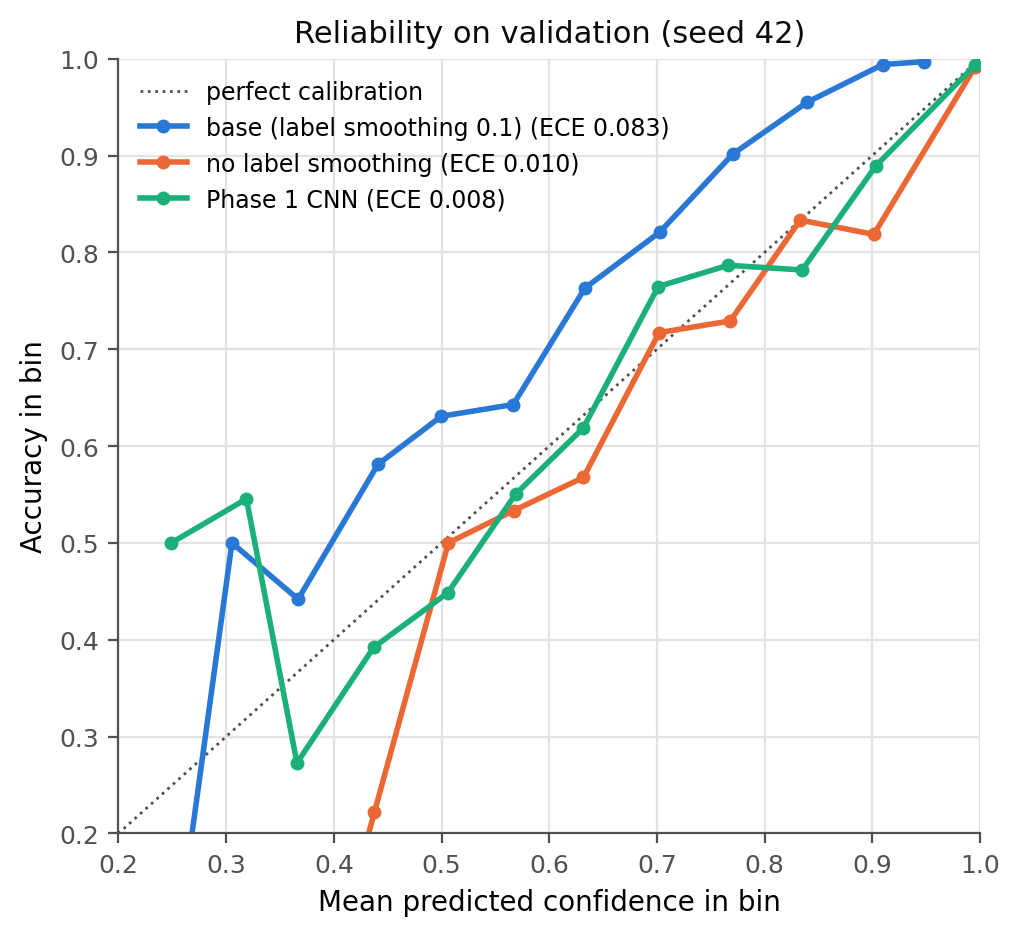
\includegraphics[width=0.85\columnwidth]{reliability.png}
\caption{Reliability diagram on validation data (seed 42). Points above the diagonal are under-confident.}
\label{fig:p2rel}
\end{figure}

\subsection{Robustness}
Table~\ref{tab:p2rob} and Fig.~\ref{fig:p2rob} show accuracy under corruption. The result is mixed.

\emph{Geometric changes.} After a 3-pixel shift the final model keeps \RobShiftF{} accuracy; the Phase 1 CNN
falls to \RobShiftP{} and H0 to \RobShiftZ. Under the largest occlusion the final model keeps \RobOcclF{}
against \RobOcclP. Random crops and random erasing train for exactly these changes.

\emph{Noise.} The final model is far more fragile than the Phase 1 CNN: \RobNoiseMidF{} against \RobNoiseMidP{} at
a noise standard deviation of 0.10, and \RobNoiseF{} against \RobNoiseP{} at 0.20. Nothing in training exposes
the network to pixel noise, and the deeper normalised network amplifies it; we did not test the cause.

\emph{Photometric changes.} Added brightness of 0.3 reduces the final model to \RobBrightF{} and the Phase 1 CNN to
\RobBrightP, while H0 stays at \RobBrightZ: gradients do not change when a constant is added. H0 is also the most
stable under reduced contrast (\RobContrastZ{} against \RobContrastF).

\emph{The fusion does not inherit this robustness.} H2 follows the deep model under every corruption
(\RobBrightH{} under brightness). The handcrafted features are valuable under photometric shift, but a fused
classifier dominated by the embedding does not use them there.

% Generated by report/build_phase2_report_assets.py. Do not edit by hand.
\begin{table*}[t]
\centering
\caption{Accuracy on corrupted test images (stratified subset of 2{,}000 images, seed 42). Level 0 is the clean subset.}
\label{tab:p2rob}
\footnotesize
\begin{tabular}{llrrrr}
\toprule
Corruption & Level & Phase 1 CNN & Final deep & H2 fusion & H0 HOG+SVM \\
\midrule
Gaussian noise (std) & 0 & 0.929 & 0.951 & 0.951 & 0.905 \\
 & 0.05 & 0.899 & 0.812 & 0.797 & 0.659 \\
 & 0.1 & 0.855 & 0.381 & 0.377 & 0.537 \\
 & 0.2 & 0.546 & 0.167 & 0.172 & 0.329 \\
\midrule
Brightness (added) & 0 & 0.929 & 0.951 & 0.951 & 0.905 \\
 & 0.1 & 0.832 & 0.786 & 0.831 & 0.898 \\
 & 0.2 & 0.575 & 0.656 & 0.713 & 0.893 \\
 & 0.3 & 0.459 & 0.553 & 0.601 & 0.890 \\
\midrule
Contrast (reduction) & 0 & 0.929 & 0.951 & 0.951 & 0.905 \\
 & 0.25 & 0.916 & 0.942 & 0.938 & 0.905 \\
 & 0.5 & 0.879 & 0.908 & 0.906 & 0.907 \\
 & 0.75 & 0.793 & 0.868 & 0.869 & 0.899 \\
\midrule
Shift (pixels) & 0 & 0.929 & 0.951 & 0.951 & 0.905 \\
 & 1 & 0.874 & 0.944 & 0.946 & 0.835 \\
 & 2 & 0.786 & 0.943 & 0.946 & 0.655 \\
 & 3 & 0.664 & 0.942 & 0.940 & 0.416 \\
\midrule
Occlusion (square side) & 0 & 0.929 & 0.951 & 0.951 & 0.905 \\
 & 5 & 0.917 & 0.949 & 0.950 & 0.896 \\
 & 8 & 0.894 & 0.935 & 0.935 & 0.872 \\
 & 11 & 0.836 & 0.916 & 0.914 & 0.794 \\
\bottomrule
\end{tabular}
\end{table*}


\begin{figure*}[t]
\centering
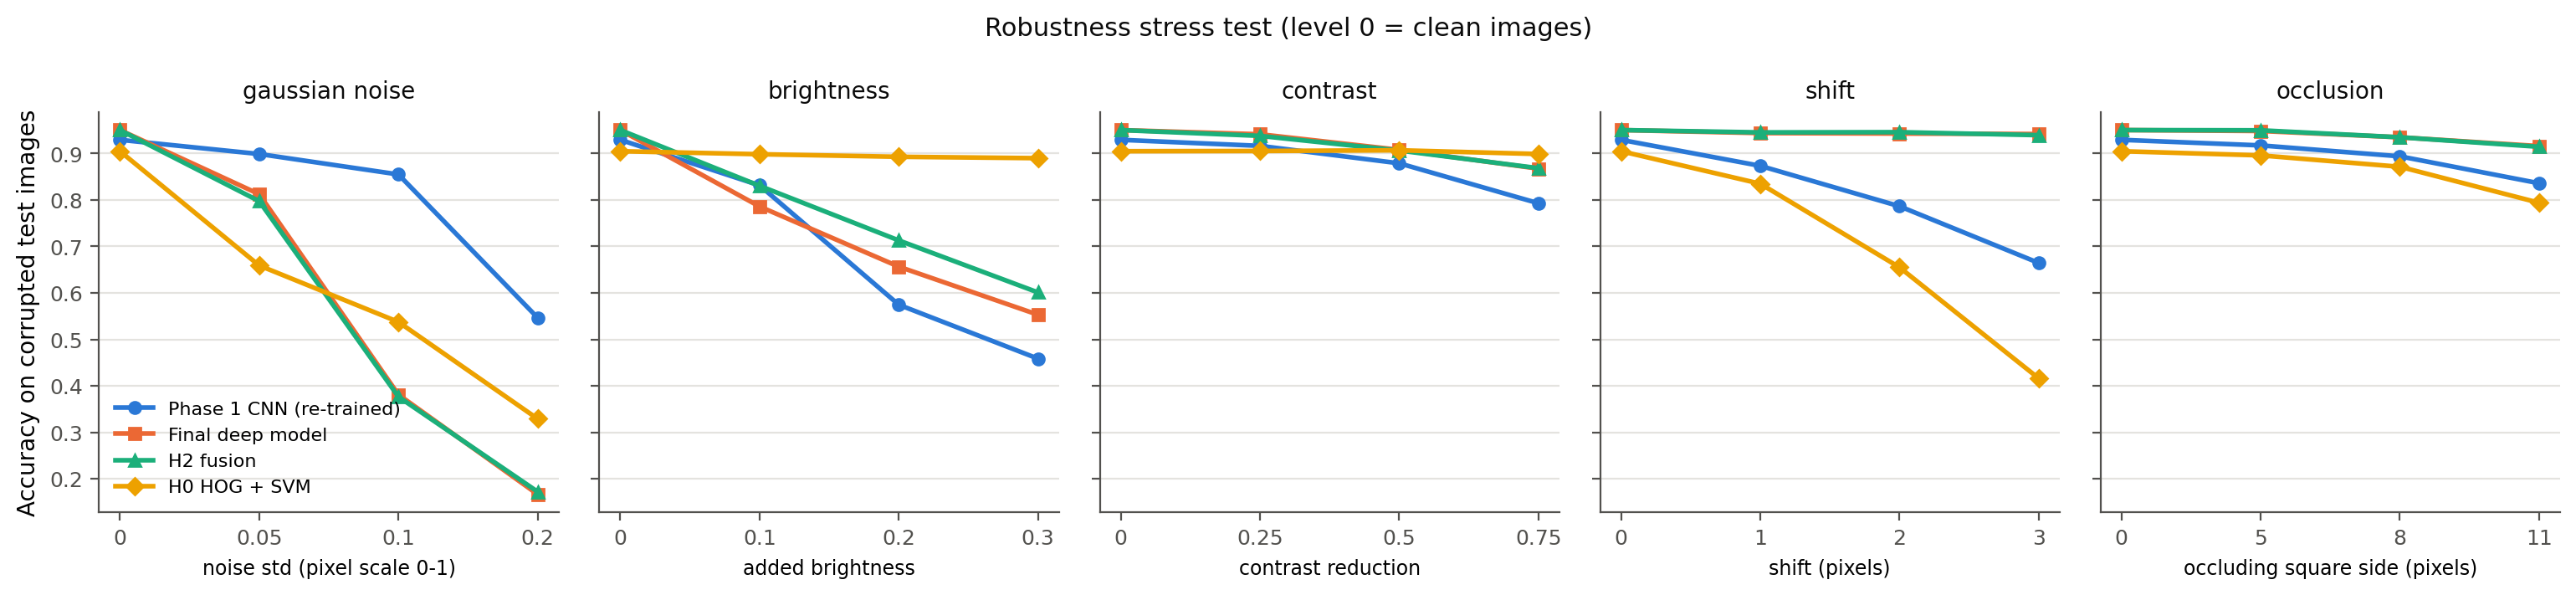
\includegraphics[width=\textwidth]{robustness.png}
\caption{Accuracy under five corruptions on a stratified subset of 2{,}000 test images (seed 42).}
\label{fig:p2rob}
\end{figure*}

\subsection{Cost}
The final model has \ParamsDeeper{} parameters against \ParamsPone{} and needs \GpuMsFinal{}~ms per image on the
GPU against \GpuMsPone{}~ms, \GpuSlowdown{} times slower (Table~\ref{tab:p2inf}); on the CPU it needs
\CpuMsFinal{}~ms against \CpuMsPone{}~ms. H2 needs \MsHtwo{}~ms per image end-to-end, dominated by HOG extraction.
The cascade pays this only for the routed \RoutedTest\% of images.

% Generated by report/build_phase2_report_assets.py. Do not edit by hand.
\begin{table}[t]
\centering
\caption{Model size and inference time per image on the Colab T4 runtime (median of repeated passes, batch size 256). The H2 row is end-to-end from raw images, including HOG extraction on the CPU.}
\label{tab:p2inf}
\footnotesize
\begin{tabular}{lrrr}
\toprule
Model & Parameters & CPU (ms) & GPU (ms) \\
\midrule
Phase 1 CNN & 241,546 & 0.50 & 0.011 \\
Final deep model & 696,042 & 2.49 & 0.077 \\
H2 fusion, end-to-end & 696,042 & 5.56 & -- \\
\bottomrule
\end{tabular}
\end{table}


% Section owners: all members (answers and limitations); Puneet (assembly)
\section{Discussion and Limitations}
\label{sec:p2discussion}
\textbf{Answers to the four questions.} (1)~The deeper residual network separates the confusable classes better:
\TestGainFinalVsPone{}~pp accuracy, Shirt recall \TestPoneShirt{} to \TestFinalShirt. The roadmap attributes the
gain to the architecture; the stronger recipe alone made the Phase 1 CNN slightly worse. (2)~Width, batch
normalisation, augmentation as a whole and the cosine schedule each account for about 0.7 to 1.1~pp; label
smoothing and random erasing for 0.2 to 0.3~pp; the horizontal flip, dropout and weight decay have no measurable
effect in this setting. (3)~Handcrafted and learned models do fail on different images, but feature-level fusion
recovers little of this: \HtwoGain{}~pp, consistent in sign and not significant. The practical value of the hybrid
work is the cascade, which matches the fusion accuracy while computing handcrafted features for \RoutedTest\% of
the images, and the observation that HOG alone is the most robust model under brightness and contrast changes.
(4)~The architecture gain is far outside both kinds of noise. It costs seven times the GPU inference time, worse
calibration and lower robustness to noise.

\textbf{Limitations.}
\begin{enumerate}
\item The test set was already used at the Phase 1 gate (Section~\ref{sec:p2protocol}).
\item Three seeds give a spread, not a significance test; McNemar tests use one seed.
\item The Phase 2 recipe was fixed in advance and not tuned. The ablations vary factors of the base model, not of
the deeper model that was finally selected; in particular, the shortcut ablation at seven layers says nothing about
thirteen.
\item One-factor ablations do not measure interactions, for example between dropout and augmentation.
\item Hybrid hyper-parameters were tuned on a 10{,}000-image subset where differences were within noise; the
selected $\alpha$ and number of HOG components lie at the edge of the grid; the SVM is fitted on embeddings of
images the CNN was trained on.
\item The robustness study uses 2{,}000 images and synthetic corruptions. It is an indication, not evidence about
photographs of real inventory.
\item Timings come from one shared cloud runtime. The run started from an uploaded archive, so the freeze file
records a timestamp and a hash but no git commit.
\item Fashion-MNIST contains ambiguous Shirt-group labels, which bounds the reachable accuracy.
\end{enumerate}

\textbf{Future work.} Temperature scaling on the validation set to restore calibration; noise and brightness
augmentation, followed by a repeat of the robustness test; out-of-fold embeddings for the hybrid; routing by input
statistics instead of confidence, so that images with unusual brightness reach the handcrafted model; and a test on
photographs taken outside the benchmark.

\section{Conclusion}
\label{sec:p2conclusion}
A thirteen-layer residual network with batch normalisation, global average pooling, augmentation and a cosine
schedule reaches \TestFinal{} $\pm$ \TestFinalStd{} test accuracy on Fashion-MNIST, \TestGainFinalVsPone{}~pp above
the Phase 1 CNN re-trained under the same protocol, with most of the gain in the upper-body classes. Controlled
ablations with three seeds identify which components matter and show that the training recipe helps only a model
with enough capacity. The handcrafted--learned fusion gives a small, consistent and statistically unsupported gain;
a confidence-gated cascade delivers the same accuracy at a fraction of its cost. The better model is less
calibrated and less robust to noise than its predecessor, which matters more for real inventory images than the
benchmark accuracy does.

\section*{Author Contributions}
M.~Selukar: architecture family, training engine, pipeline integration, experiments on the GPU.
A.~Singh: hybrid models, controls and cascade.
A.~Sharma: augmentation pipeline and robustness study.
T.~Rao: ablation design, regularisation analysis and model selection stage.
R.~Kumar: multi-seed statistics, significance tests, calibration and error analysis.
P.~Takhar: experiment configuration, run store, freeze and test gate, reporting and literature review.
All authors wrote the sections on their components and reviewed the manuscript.


\bibliographystyle{IEEEtran}
\bibliography{references}

\end{document}
